% Options for packages loaded elsewhere
\PassOptionsToPackage{unicode}{hyperref}
\PassOptionsToPackage{hyphens}{url}
%
\documentclass[
]{article}
\usepackage{amsmath,amssymb}
\usepackage{lmodern}
\usepackage{iftex}
\ifPDFTeX
  \usepackage[T1]{fontenc}
  \usepackage[utf8]{inputenc}
  \usepackage{textcomp} % provide euro and other symbols
\else % if luatex or xetex
  \usepackage{unicode-math}
  \defaultfontfeatures{Scale=MatchLowercase}
  \defaultfontfeatures[\rmfamily]{Ligatures=TeX,Scale=1}
\fi
% Use upquote if available, for straight quotes in verbatim environments
\IfFileExists{upquote.sty}{\usepackage{upquote}}{}
\IfFileExists{microtype.sty}{% use microtype if available
  \usepackage[]{microtype}
  \UseMicrotypeSet[protrusion]{basicmath} % disable protrusion for tt fonts
}{}
\makeatletter
\@ifundefined{KOMAClassName}{% if non-KOMA class
  \IfFileExists{parskip.sty}{%
    \usepackage{parskip}
  }{% else
    \setlength{\parindent}{0pt}
    \setlength{\parskip}{6pt plus 2pt minus 1pt}}
}{% if KOMA class
  \KOMAoptions{parskip=half}}
\makeatother
\usepackage{xcolor}
\usepackage[margin=1in]{geometry}
\usepackage{color}
\usepackage{fancyvrb}
\newcommand{\VerbBar}{|}
\newcommand{\VERB}{\Verb[commandchars=\\\{\}]}
\DefineVerbatimEnvironment{Highlighting}{Verbatim}{commandchars=\\\{\}}
% Add ',fontsize=\small' for more characters per line
\usepackage{framed}
\definecolor{shadecolor}{RGB}{248,248,248}
\newenvironment{Shaded}{\begin{snugshade}}{\end{snugshade}}
\newcommand{\AlertTok}[1]{\textcolor[rgb]{0.94,0.16,0.16}{#1}}
\newcommand{\AnnotationTok}[1]{\textcolor[rgb]{0.56,0.35,0.01}{\textbf{\textit{#1}}}}
\newcommand{\AttributeTok}[1]{\textcolor[rgb]{0.77,0.63,0.00}{#1}}
\newcommand{\BaseNTok}[1]{\textcolor[rgb]{0.00,0.00,0.81}{#1}}
\newcommand{\BuiltInTok}[1]{#1}
\newcommand{\CharTok}[1]{\textcolor[rgb]{0.31,0.60,0.02}{#1}}
\newcommand{\CommentTok}[1]{\textcolor[rgb]{0.56,0.35,0.01}{\textit{#1}}}
\newcommand{\CommentVarTok}[1]{\textcolor[rgb]{0.56,0.35,0.01}{\textbf{\textit{#1}}}}
\newcommand{\ConstantTok}[1]{\textcolor[rgb]{0.00,0.00,0.00}{#1}}
\newcommand{\ControlFlowTok}[1]{\textcolor[rgb]{0.13,0.29,0.53}{\textbf{#1}}}
\newcommand{\DataTypeTok}[1]{\textcolor[rgb]{0.13,0.29,0.53}{#1}}
\newcommand{\DecValTok}[1]{\textcolor[rgb]{0.00,0.00,0.81}{#1}}
\newcommand{\DocumentationTok}[1]{\textcolor[rgb]{0.56,0.35,0.01}{\textbf{\textit{#1}}}}
\newcommand{\ErrorTok}[1]{\textcolor[rgb]{0.64,0.00,0.00}{\textbf{#1}}}
\newcommand{\ExtensionTok}[1]{#1}
\newcommand{\FloatTok}[1]{\textcolor[rgb]{0.00,0.00,0.81}{#1}}
\newcommand{\FunctionTok}[1]{\textcolor[rgb]{0.00,0.00,0.00}{#1}}
\newcommand{\ImportTok}[1]{#1}
\newcommand{\InformationTok}[1]{\textcolor[rgb]{0.56,0.35,0.01}{\textbf{\textit{#1}}}}
\newcommand{\KeywordTok}[1]{\textcolor[rgb]{0.13,0.29,0.53}{\textbf{#1}}}
\newcommand{\NormalTok}[1]{#1}
\newcommand{\OperatorTok}[1]{\textcolor[rgb]{0.81,0.36,0.00}{\textbf{#1}}}
\newcommand{\OtherTok}[1]{\textcolor[rgb]{0.56,0.35,0.01}{#1}}
\newcommand{\PreprocessorTok}[1]{\textcolor[rgb]{0.56,0.35,0.01}{\textit{#1}}}
\newcommand{\RegionMarkerTok}[1]{#1}
\newcommand{\SpecialCharTok}[1]{\textcolor[rgb]{0.00,0.00,0.00}{#1}}
\newcommand{\SpecialStringTok}[1]{\textcolor[rgb]{0.31,0.60,0.02}{#1}}
\newcommand{\StringTok}[1]{\textcolor[rgb]{0.31,0.60,0.02}{#1}}
\newcommand{\VariableTok}[1]{\textcolor[rgb]{0.00,0.00,0.00}{#1}}
\newcommand{\VerbatimStringTok}[1]{\textcolor[rgb]{0.31,0.60,0.02}{#1}}
\newcommand{\WarningTok}[1]{\textcolor[rgb]{0.56,0.35,0.01}{\textbf{\textit{#1}}}}
\usepackage{graphicx}
\makeatletter
\def\maxwidth{\ifdim\Gin@nat@width>\linewidth\linewidth\else\Gin@nat@width\fi}
\def\maxheight{\ifdim\Gin@nat@height>\textheight\textheight\else\Gin@nat@height\fi}
\makeatother
% Scale images if necessary, so that they will not overflow the page
% margins by default, and it is still possible to overwrite the defaults
% using explicit options in \includegraphics[width, height, ...]{}
\setkeys{Gin}{width=\maxwidth,height=\maxheight,keepaspectratio}
% Set default figure placement to htbp
\makeatletter
\def\fps@figure{htbp}
\makeatother
\setlength{\emergencystretch}{3em} % prevent overfull lines
\providecommand{\tightlist}{%
  \setlength{\itemsep}{0pt}\setlength{\parskip}{0pt}}
\setcounter{secnumdepth}{-\maxdimen} % remove section numbering
\ifLuaTeX
  \usepackage{selnolig}  % disable illegal ligatures
\fi
\IfFileExists{bookmark.sty}{\usepackage{bookmark}}{\usepackage{hyperref}}
\IfFileExists{xurl.sty}{\usepackage{xurl}}{} % add URL line breaks if available
\urlstyle{same} % disable monospaced font for URLs
\hypersetup{
  pdftitle={Practical Work 3 - Regularised Regression Methods},
  pdfauthor={Adib Habbou - Alae Khidour},
  hidelinks,
  pdfcreator={LaTeX via pandoc}}

\title{Practical Work 3 - Regularised Regression Methods}
\author{Adib Habbou - Alae Khidour}
\date{07-11-2022}

\begin{document}
\maketitle

\hypertarget{data-analysis}{%
\section{Data Analysis}\label{data-analysis}}

\hypertarget{data-import}{%
\subsection{Data Import}\label{data-import}}

\begin{Shaded}
\begin{Highlighting}[]
\NormalTok{diabetes\_data }\OtherTok{\textless{}{-}} \FunctionTok{read.table}\NormalTok{(}\AttributeTok{file =} \StringTok{"diabetes.txt"}\NormalTok{,}\AttributeTok{header =} \ConstantTok{TRUE}\NormalTok{)}
\end{Highlighting}
\end{Shaded}

\hypertarget{data-conversion}{%
\subsection{Data Conversion}\label{data-conversion}}

\begin{Shaded}
\begin{Highlighting}[]
\NormalTok{YBin }\OtherTok{\textless{}{-}} \FunctionTok{as.numeric}\NormalTok{(diabetes\_data}\SpecialCharTok{$}\NormalTok{Y }\SpecialCharTok{\textgreater{}} \FunctionTok{median}\NormalTok{(diabetes\_data}\SpecialCharTok{$}\NormalTok{Y))}
\NormalTok{diabetes\_data }\OtherTok{\textless{}{-}}\NormalTok{ diabetes\_data[,}\SpecialCharTok{{-}}\DecValTok{11}\NormalTok{]}
\NormalTok{diabetes\_data }\OtherTok{\textless{}{-}} \FunctionTok{cbind}\NormalTok{(diabetes\_data, YBin)}
\end{Highlighting}
\end{Shaded}

\begin{Shaded}
\begin{Highlighting}[]
\FunctionTok{head}\NormalTok{(diabetes\_data)}
\end{Highlighting}
\end{Shaded}

\begin{verbatim}
  AGE SEX  BMI  BP  S1    S2 S3 S4     S5 S6 YBin
1  59   2 32.1 101 157  93.2 38  4 4.8598 87    1
2  48   1 21.6  87 183 103.2 70  3 3.8918 69    0
3  72   2 30.5  93 156  93.6 41  4 4.6728 85    1
4  24   1 25.3  84 198 131.4 40  5 4.8903 89    1
5  50   1 23.0 101 192 125.4 52  4 4.2905 80    0
6  23   1 22.6  89 139  64.8 61  2 4.1897 68    0
\end{verbatim}

\hypertarget{data-visualization}{%
\subsection{Data Visualization}\label{data-visualization}}

\begin{Shaded}
\begin{Highlighting}[]
\FunctionTok{pairs}\NormalTok{(diabetes\_data, }\AttributeTok{pch =} \DecValTok{22}\NormalTok{, }\AttributeTok{bg =} \FunctionTok{c}\NormalTok{(}\StringTok{"tomato1"}\NormalTok{,}\StringTok{"royalblue3"}\NormalTok{)[}\FunctionTok{unclass}\NormalTok{(}\FunctionTok{factor}\NormalTok{(diabetes\_data[,}\StringTok{"YBin"}\NormalTok{]))])}
\end{Highlighting}
\end{Shaded}

\begin{center}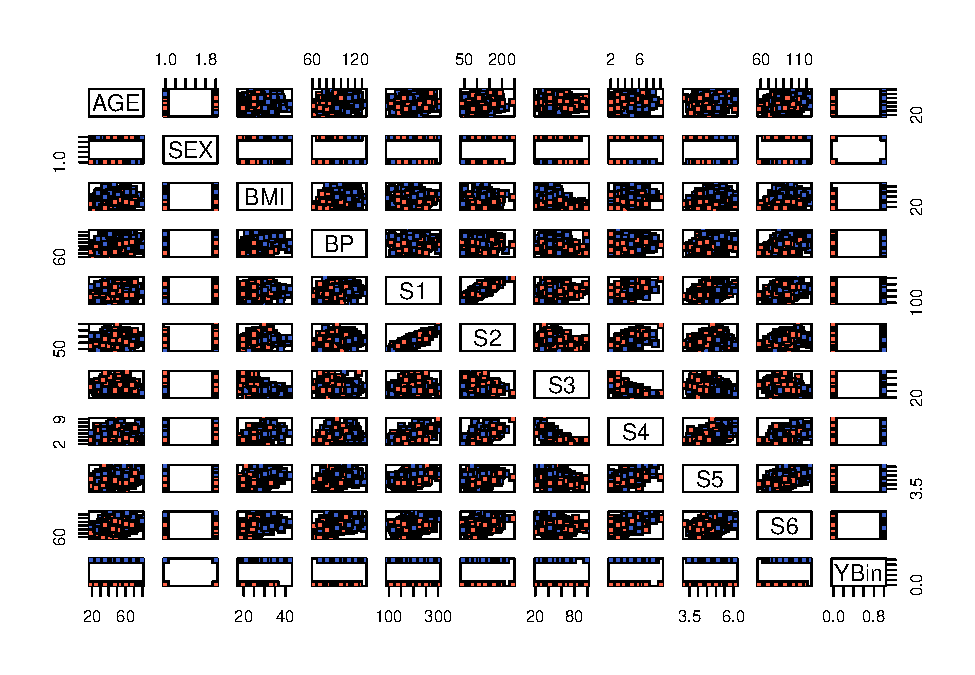
\includegraphics{TP3_MERR_HABBOU_KHIDOUR_files/figure-latex/unnamed-chunk-4-1} \end{center}

Red squares correspond to observations where \(YBin\) is equal to 0
which means \(Y\) is lower than the median.

Blue squares correspond to observations where \(YBin\) is equal to 1
which means \(Y\) is greater than the median.

From the above plot, we observe the following:

\begin{itemize}
\item
  Colinearity between \(S1\) and \(S2\)
\item
  Above a certain value for \(BMI\) and \(BP\) we find only blue squares
\end{itemize}

\hypertarget{study-of-correlation}{%
\subsection{Study of correlation}\label{study-of-correlation}}

\begin{Shaded}
\begin{Highlighting}[]
\NormalTok{corr }\OtherTok{\textless{}{-}} \FunctionTok{cor}\NormalTok{(diabetes\_data)}
\FunctionTok{corrplot}\NormalTok{(corr, }\AttributeTok{method =} \StringTok{"circle"}\NormalTok{)}
\end{Highlighting}
\end{Shaded}

\begin{center}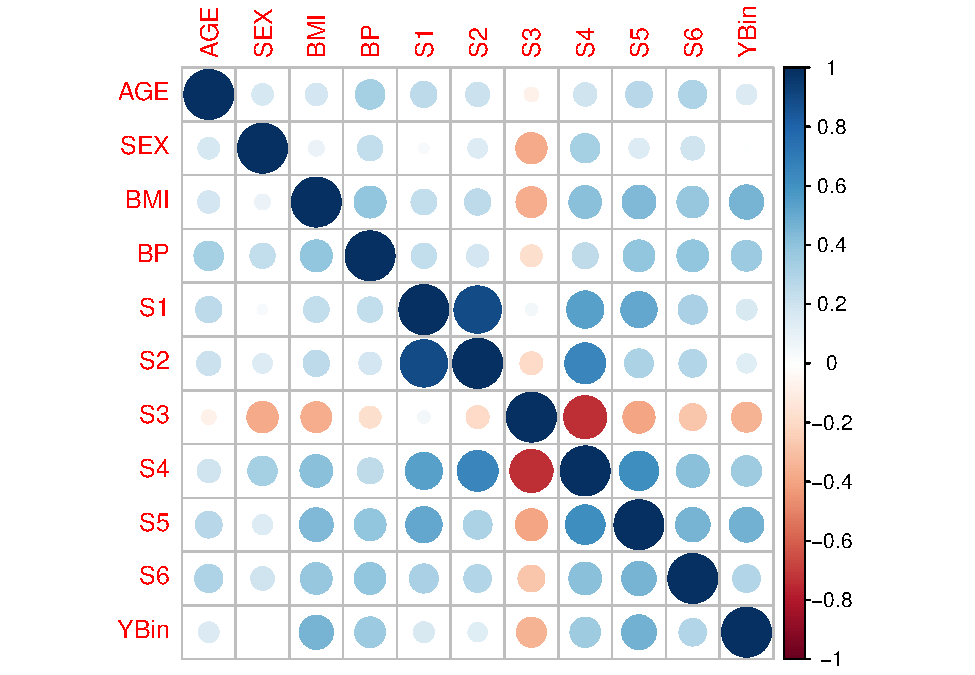
\includegraphics{TP3_MERR_HABBOU_KHIDOUR_files/figure-latex/unnamed-chunk-5-1} \end{center}

The correlation plot provides us with a lot of information such as:

\begin{itemize}
\item
  S1 and S2 are highly positively correlated;
\item
  S3 and S4 are highly negatively correlated.
\end{itemize}

We need to keep in mind the correlation between our variables.

The potential colinearity between variables can have an impact on the
Standard Error.

More than that, it means that the co-variable signifacitivity test is
useless.

\hypertarget{logistic-regression}{%
\section{Logistic Regression}\label{logistic-regression}}

\hypertarget{data-partitionning}{%
\subsection{Data Partitionning}\label{data-partitionning}}

\begin{Shaded}
\begin{Highlighting}[]
\NormalTok{sample }\OtherTok{\textless{}{-}} \FunctionTok{sample}\NormalTok{(}\FunctionTok{c}\NormalTok{(}\ConstantTok{TRUE}\NormalTok{, }\ConstantTok{FALSE}\NormalTok{), }\FunctionTok{nrow}\NormalTok{(diabetes\_data), }\AttributeTok{replace =} \ConstantTok{TRUE}\NormalTok{, }\AttributeTok{prob =} \FunctionTok{c}\NormalTok{(}\FloatTok{0.8}\NormalTok{, }\FloatTok{0.2}\NormalTok{))}
\NormalTok{train\_data }\OtherTok{\textless{}{-}}\NormalTok{ diabetes\_data[sample, ]}
\NormalTok{test\_data }\OtherTok{\textless{}{-}}\NormalTok{ diabetes\_data[}\SpecialCharTok{!}\NormalTok{sample, ]}
\end{Highlighting}
\end{Shaded}

\hypertarget{application-of-logistic-regression}{%
\subsection{Application of logistic
regression}\label{application-of-logistic-regression}}

\begin{Shaded}
\begin{Highlighting}[]
\NormalTok{reg\_log }\OtherTok{=} \FunctionTok{glm}\NormalTok{(}\AttributeTok{formula =}\NormalTok{ YBin }\SpecialCharTok{\textasciitilde{}}\NormalTok{ ., }\AttributeTok{family =}\NormalTok{ binomial, }\AttributeTok{data =}\NormalTok{ train\_data)}
\FunctionTok{summary}\NormalTok{(reg\_log)}
\end{Highlighting}
\end{Shaded}

\begin{verbatim}

Call:
glm(formula = YBin ~ ., family = binomial, data = train_data)

Deviance Residuals: 
    Min       1Q   Median       3Q      Max  
-2.3682  -0.7258  -0.2290   0.7858   2.2469  

Coefficients:
              Estimate Std. Error z value Pr(>|z|)    
(Intercept) -12.556955   4.201986  -2.988 0.002805 ** 
AGE           0.006159   0.011294   0.545 0.585552    
SEX          -1.196829   0.330552  -3.621 0.000294 ***
BMI           0.145721   0.040425   3.605 0.000313 ***
BP            0.035889   0.011711   3.064 0.002181 ** 
S1           -0.036586   0.035868  -1.020 0.307709    
S2            0.025692   0.034528   0.744 0.456817    
S3           -0.017178   0.048020  -0.358 0.720550    
S4           -0.058585   0.335076  -0.175 0.861204    
S5            2.574305   0.970770   2.652 0.008006 ** 
S6           -0.001680   0.014943  -0.112 0.910472    
---
Signif. codes:  0 '***' 0.001 '**' 0.01 '*' 0.05 '.' 0.1 ' ' 1

(Dispersion parameter for binomial family taken to be 1)

    Null deviance: 491.66  on 354  degrees of freedom
Residual deviance: 337.97  on 344  degrees of freedom
AIC: 359.97

Number of Fisher Scoring iterations: 5
\end{verbatim}

\begin{itemize}
\item
  For the Deviance Residuals we observe that they are close to be
  centered on 0 and roughly symmetrical.
\item
  We can make assumptions on the significativity of the co-variables by
  looking at their p-values. For example \(BMI\) and \(S5\) are highly
  significant co-variables for our model meanwhile \(AGE\) and \(S4\)
  are less significant.
\item
  The dispersion parameter in our case is equal to 1, but we can adjust
  it if we want too. Since we are not estimating the variance from the
  data instead we are just deriving it from the mean, it is possible
  that the variance is underestimated.
\item
  The Akaike Information Criterion \(AIC\) will help us to compare
  between different models.
\item
  The number of Fisher Scoring iterations tells us how quickly the
  function converges to the maximum likelihood estimated for the
  coefficients.
\end{itemize}

\hypertarget{study-of-the-coefficients}{%
\subsection{Study of the coefficients}\label{study-of-the-coefficients}}

\begin{Shaded}
\begin{Highlighting}[]
\NormalTok{reg\_log}\SpecialCharTok{$}\NormalTok{coefficients}
\end{Highlighting}
\end{Shaded}

\begin{verbatim}
  (Intercept)           AGE           SEX           BMI            BP 
-12.556955467   0.006158551  -1.196829362   0.145720525   0.035888783 
           S1            S2            S3            S4            S5 
 -0.036586335   0.025692333  -0.017177982  -0.058585076   2.574305138 
           S6 
 -0.001680268 
\end{verbatim}

We should also not look at the estimated value of the coefficient to
determine co-variable significativity because even a very low estimated
coefficient can become bigger at the end depending on the co-variable
unit and magnitude.

The most significant co-variable is \(S5\), the less significant
co-variable is \(AGE\). But we need to keep in mind that it does not
mean that \(AGE\) is not significant in reality, it is just the least
significant in our model according to the computed p-values.

\hypertarget{predictions}{%
\subsection{Predictions}\label{predictions}}

\begin{Shaded}
\begin{Highlighting}[]
\NormalTok{predict\_response }\OtherTok{\textless{}{-}} \FunctionTok{predict.glm}\NormalTok{(reg\_log, }\AttributeTok{newdata =}\NormalTok{ test\_data, }\AttributeTok{type =} \StringTok{"response"}\NormalTok{)}
\NormalTok{predict\_response}
\end{Highlighting}
\end{Shaded}

\begin{verbatim}
         1          3          7         15         28         62         76 
0.86329467 0.71504642 0.06986510 0.17789728 0.69906081 0.68590014 0.30483918 
        81         93        100        116        126        129        130 
0.67245356 0.77091651 0.50841331 0.67962513 0.81373564 0.17911270 0.86677859 
       136        138        140        147        151        153        159 
0.95983236 0.94754393 0.97724965 0.70233490 0.88955594 0.71051854 0.15687751 
       161        165        168        174        176        177        179 
0.16221270 0.43353679 0.97549457 0.18732964 0.38277043 0.45826033 0.14279764 
       183        189        197        199        211        212        219 
0.58434920 0.49057045 0.13359714 0.46824109 0.27515895 0.77536362 0.47429181 
       222        223        227        238        246        250        256 
0.57077522 0.55706512 0.06531666 0.07278593 0.23283050 0.95671317 0.31723787 
       262        266        269        270        271        275        278 
0.21314932 0.28138917 0.91416497 0.08307716 0.74546137 0.77527641 0.27650813 
       279        283        290        308        314        319        322 
0.23198144 0.37841974 0.69457652 0.42961912 0.84663172 0.59910781 0.98608323 
       326        328        331        339        345        349        350 
0.88053458 0.89685322 0.60060210 0.37807450 0.43605796 0.32609070 0.19828026 
       352        355        366        368        372        375        379 
0.09927780 0.66552849 0.65706426 0.92545745 0.82309033 0.43871947 0.62384277 
       380        383        386        390        394        398        401 
0.47891664 0.97732092 0.40891224 0.05695007 0.19724775 0.83915554 0.67137916 
       411        413        421        429        433        434        436 
0.58085699 0.91386715 0.45108044 0.94314186 0.87476549 0.02922132 0.33445492 
       438        440        441 
0.80538600 0.25758890 0.89778089 
\end{verbatim}

Using the type \(response\) we obtain values between 0 and 1 which
correspond to the probability of \(YBin\) being equal to 1 computed from
the area under the link function.

\begin{Shaded}
\begin{Highlighting}[]
\NormalTok{predict\_link }\OtherTok{\textless{}{-}} \FunctionTok{predict.glm}\NormalTok{(reg\_log, }\AttributeTok{newdata =}\NormalTok{ test\_data, }\AttributeTok{type =} \StringTok{"link"}\NormalTok{)}
\NormalTok{predict\_link}
\end{Highlighting}
\end{Shaded}

\begin{verbatim}
          1           3           7          15          28          62 
 1.84292834  0.92002120 -2.58876336 -1.53065904  0.84282952  0.78102107 
         76          81          93         100         116         126 
-0.82435886  0.71930323  1.21349356  0.03365640  0.75204961  1.47446858 
        129         130         136         138         140         147 
-1.52237059  1.87277112  3.17369698  2.89389719  3.76016160  0.85844134 
        151         153         159         161         165         168 
 2.08621329  0.89790381 -1.68164694 -1.64185581 -0.26743549  3.68405001 
        174         176         177         179         183         189 
-1.46745570 -0.47780562 -0.16734816 -1.79224550  0.34065327 -0.03772266 
        197         199         211         212         219         222 
-1.86952110 -0.12720690 -0.96860347  1.23884908 -0.10292351  0.28501472 
        223         227         238         246         250         256 
 0.22925940 -2.66096059 -2.54466183 -1.19239706  3.09565521 -0.76649467 
        262         266         269         270         271         275 
-1.30604555 -0.93758127  2.36558387 -2.40125354  1.07455071  1.23834848 
        278         279         283         290         308         314 
-0.96184907 -1.19715651 -0.49626104  0.82160304 -0.28340528  1.70842367 
        319         322         326         328         331         339 
 0.40174902  4.26064607  1.99750226  2.16273914  0.40797451 -0.49772907 
        345         349         350         352         355         366 
-0.25717633 -0.72591998 -1.39707764 -2.20527495  0.68802974  0.65023875 
        368         372         375         379         380         383 
 2.51891804  1.53742669 -0.24636064  0.50589116 -0.08438348  3.76337211 
        386         390         394         398         401         411 
-0.36846392 -2.80694427 -1.40358561  1.65195826  0.71442940  0.32629243 
        413         421         429         433         434         436 
 2.36179428 -0.19630624  2.80865738  1.94376782 -3.50319992 -0.68810429 
        438         440         441 
 1.42030358 -1.05853825  2.17280735 
\end{verbatim}

Using the type \(link\) we obtain values of the link function.

\hypertarget{odd-ratios}{%
\subsection{Odd-Ratios}\label{odd-ratios}}

\begin{Shaded}
\begin{Highlighting}[]
\FunctionTok{exp}\NormalTok{(}\FunctionTok{coef}\NormalTok{(reg\_log))}
\end{Highlighting}
\end{Shaded}

\begin{verbatim}
 (Intercept)          AGE          SEX          BMI           BP           S1 
3.520331e-06 1.006178e+00 3.021507e-01 1.156873e+00 1.036541e+00 9.640749e-01 
          S2           S3           S4           S5           S6 
1.026025e+00 9.829687e-01 9.430980e-01 1.312220e+01 9.983211e-01 
\end{verbatim}

From the odd-ratios obtained for each co-variable we can evaluate the
influence of the co-variable on the target knowing that:

\begin{itemize}
\item
  When the Odd-Ratio is lower than 1 it means that the co-variable had a
  negative influence on the target, for instance \(AGE\), \(SEX\),
  \(S1\), \(S3\), \(S4\) and \(S6\).
\item
  When the Odd-Ratio is greater than 1 it means that the co-variable had
  a positive influence on the target, for instance \(BMI\), \(BP\) and
  \(S2\).
\end{itemize}

The limits of this approach is that if we change the binary labels we
had (0 and 1 for our case) we will obtain different values for the
estimated coefficients.

\hypertarget{performance}{%
\subsection{Performance}\label{performance}}

\hypertarget{map}{%
\subsubsection{MAP}\label{map}}

\begin{Shaded}
\begin{Highlighting}[]
\NormalTok{prediction }\OtherTok{\textless{}{-}} \FunctionTok{as.numeric}\NormalTok{(}\FunctionTok{predict.glm}\NormalTok{(reg\_log, }\AttributeTok{newdata =}\NormalTok{ diabetes\_data, }\AttributeTok{type =} \StringTok{"response"}\NormalTok{) }\SpecialCharTok{\textgreater{}} \FloatTok{0.5}\NormalTok{)}
\end{Highlighting}
\end{Shaded}

Using the Maximum A Posteriori criteria we can make predictions for our
binary variable \(YBin\):

\begin{Shaded}
\begin{Highlighting}[]
\FunctionTok{table}\NormalTok{(prediction)}
\end{Highlighting}
\end{Shaded}

\begin{verbatim}
prediction
  0   1 
223 219 
\end{verbatim}

Knowing that our target variable have the following values:

\begin{Shaded}
\begin{Highlighting}[]
\FunctionTok{table}\NormalTok{(diabetes\_data}\SpecialCharTok{$}\NormalTok{YBin)}
\end{Highlighting}
\end{Shaded}

\begin{verbatim}

  0   1 
221 221 
\end{verbatim}

By comparing the both tables we can tell that our predictions are quite
consistent, since our model has nearly the same count for 0 and 1 than
the target variable in our data set.

\hypertarget{confusion-matrix}{%
\subsubsection{Confusion Matrix}\label{confusion-matrix}}

\begin{Shaded}
\begin{Highlighting}[]
\NormalTok{confusion\_matrix }\OtherTok{\textless{}{-}} \FunctionTok{table}\NormalTok{(diabetes\_data}\SpecialCharTok{$}\NormalTok{YBin, prediction)}
\NormalTok{confusion\_matrix}
\end{Highlighting}
\end{Shaded}

\begin{verbatim}
   prediction
      0   1
  0 166  55
  1  57 164
\end{verbatim}

Here we just computed the confusion matrix for our model. This matrix
has 4 values which corresponds respectively to the number of TRUE
NEGATIVE, FALSE NEGATIVE, FALSE POSITIVE and TRUE POSTIVE.

\begin{itemize}
\item
  TRUE NEGATIVE: specificity which is the ability to predict
  \(\hat{YBin} = 0\) for \(YBin = 0\)
\item
  TRUE POSITIVE: sensitivity which is ability to predict
  \(\hat{YBin} = 1\) for \(YBin = 1\)
\end{itemize}

\hypertarget{accuracy}{%
\subsubsection{Accuracy}\label{accuracy}}

\begin{Shaded}
\begin{Highlighting}[]
\NormalTok{accuracy }\OtherTok{\textless{}{-}}\NormalTok{ (confusion\_matrix[}\DecValTok{1}\NormalTok{,}\DecValTok{1}\NormalTok{] }\SpecialCharTok{+}\NormalTok{ confusion\_matrix[}\DecValTok{2}\NormalTok{,}\DecValTok{2}\NormalTok{]) }\SpecialCharTok{/} \FunctionTok{nrow}\NormalTok{(diabetes\_data)}
\NormalTok{accuracy}
\end{Highlighting}
\end{Shaded}

\begin{verbatim}
[1] 0.7466063
\end{verbatim}

The accuracy of our model correspond to it's ability to predict the
right value (O or 1) for all the observations of our data set. In our
case it's equal to \(76\,\%\).

\hypertarget{gloabl-error}{%
\subsubsection{Gloabl Error}\label{gloabl-error}}

\begin{Shaded}
\begin{Highlighting}[]
\NormalTok{global\_error }\OtherTok{\textless{}{-}}\NormalTok{ (confusion\_matrix[}\DecValTok{1}\NormalTok{,}\DecValTok{2}\NormalTok{] }\SpecialCharTok{+}\NormalTok{ confusion\_matrix[}\DecValTok{2}\NormalTok{,}\DecValTok{1}\NormalTok{]) }\SpecialCharTok{/} \FunctionTok{nrow}\NormalTok{(diabetes\_data)}
\NormalTok{global\_error}
\end{Highlighting}
\end{Shaded}

\begin{verbatim}
[1] 0.2533937
\end{verbatim}

The global error of our model correspond to it's inability to predict
the right value (O or 1) for all the observations of our data set. In
our case it's equal to \(24\,\%\).

\hypertarget{recall}{%
\subsubsection{Recall}\label{recall}}

\begin{Shaded}
\begin{Highlighting}[]
\NormalTok{recall }\OtherTok{\textless{}{-}}\NormalTok{ confusion\_matrix[}\DecValTok{2}\NormalTok{,}\DecValTok{2}\NormalTok{] }\SpecialCharTok{/}\NormalTok{ (confusion\_matrix[}\DecValTok{1}\NormalTok{,}\DecValTok{2}\NormalTok{] }\SpecialCharTok{+}\NormalTok{ confusion\_matrix[}\DecValTok{2}\NormalTok{,}\DecValTok{2}\NormalTok{])}
\NormalTok{recall}
\end{Highlighting}
\end{Shaded}

\begin{verbatim}
[1] 0.7488584
\end{verbatim}

The recall of our model correspond to the correctly predicted positive
rate. In our case it's equal to \(75\,\%\).

\hypertarget{precision}{%
\subsubsection{Precision}\label{precision}}

\begin{Shaded}
\begin{Highlighting}[]
\NormalTok{precision }\OtherTok{\textless{}{-}}\NormalTok{ confusion\_matrix[}\DecValTok{2}\NormalTok{,}\DecValTok{2}\NormalTok{] }\SpecialCharTok{/}\NormalTok{ (confusion\_matrix[}\DecValTok{2}\NormalTok{,}\DecValTok{1}\NormalTok{] }\SpecialCharTok{+}\NormalTok{ confusion\_matrix[}\DecValTok{2}\NormalTok{,}\DecValTok{2}\NormalTok{])}
\NormalTok{precision}
\end{Highlighting}
\end{Shaded}

\begin{verbatim}
[1] 0.7420814
\end{verbatim}

The precision of our model correspond to the rate of correct positive
predictions. In our case it's equal to \(78\,\%\).

\hypertarget{f1-score}{%
\subsubsection{F1-Score}\label{f1-score}}

\begin{Shaded}
\begin{Highlighting}[]
\NormalTok{f1\_score }\OtherTok{\textless{}{-}}\NormalTok{ (}\DecValTok{2} \SpecialCharTok{*}\NormalTok{ precision }\SpecialCharTok{*}\NormalTok{ recall) }\SpecialCharTok{/}\NormalTok{ (precision }\SpecialCharTok{+}\NormalTok{ recall)}
\NormalTok{f1\_score}
\end{Highlighting}
\end{Shaded}

\begin{verbatim}
[1] 0.7454545
\end{verbatim}

The F1-score correspond to the ability of our model to predict positive
individuals well. In our case it's equal to \(76\,\%\).

The \(F_\beta\)-score uses a more general formula where \(\beta\) is
chosen such that recall is considered \(\beta\) times as important as
precision.

\[F_\beta = \frac{(1 + \beta^2) * precision * recall}{(\beta^2 * precision) + recall}\]

\hypertarget{false-positive-rate}{%
\subsubsection{False Positive Rate}\label{false-positive-rate}}

\begin{Shaded}
\begin{Highlighting}[]
\NormalTok{confusion\_matrix[}\DecValTok{2}\NormalTok{,}\DecValTok{1}\NormalTok{] }\SpecialCharTok{/} \FunctionTok{nrow}\NormalTok{(diabetes\_data)}
\end{Highlighting}
\end{Shaded}

\begin{verbatim}
[1] 0.1289593
\end{verbatim}

The false positive is equal to \(11\,\%\).

\hypertarget{false-negative-rate}{%
\subsubsection{False Negative Rate}\label{false-negative-rate}}

\begin{Shaded}
\begin{Highlighting}[]
\NormalTok{confusion\_matrix[}\DecValTok{1}\NormalTok{,}\DecValTok{2}\NormalTok{] }\SpecialCharTok{/} \FunctionTok{nrow}\NormalTok{(diabetes\_data)}
\end{Highlighting}
\end{Shaded}

\begin{verbatim}
[1] 0.1244344
\end{verbatim}

The false negative is equal to \(13\,\%\).

\hypertarget{k-fold}{%
\subsubsection{K-Fold}\label{k-fold}}

\begin{Shaded}
\begin{Highlighting}[]
\NormalTok{kfold\_all }\OtherTok{\textless{}{-}} \ControlFlowTok{function}\NormalTok{(k) }\CommentTok{\# k is here the number of folds}
\NormalTok{\{}
  \CommentTok{\# create a vector of length number of folds}
\NormalTok{  performance }\OtherTok{\textless{}{-}} \FunctionTok{vector}\NormalTok{(}\AttributeTok{length =}\NormalTok{ k)}
  \CommentTok{\# create a sequence from 1 to k}
\NormalTok{  folds }\OtherTok{\textless{}{-}} \FunctionTok{cut}\NormalTok{(}\FunctionTok{seq}\NormalTok{(}\DecValTok{1}\NormalTok{,}\FunctionTok{nrow}\NormalTok{(diabetes\_data)), }\AttributeTok{breaks =}\NormalTok{ k, }\AttributeTok{labels =} \ConstantTok{FALSE}\NormalTok{)}
  \CommentTok{\# perform k fold cross validation}
  \ControlFlowTok{for}\NormalTok{(i }\ControlFlowTok{in} \DecValTok{1}\SpecialCharTok{:}\NormalTok{k)}
\NormalTok{  \{}
    \CommentTok{\# split data by fold}
\NormalTok{    index }\OtherTok{\textless{}{-}} \FunctionTok{which}\NormalTok{(folds }\SpecialCharTok{==}\NormalTok{ i, }\AttributeTok{arr.ind =} \ConstantTok{TRUE}\NormalTok{)}
\NormalTok{    test\_data }\OtherTok{\textless{}{-}}\NormalTok{ diabetes\_data[index,]}
\NormalTok{    train\_data }\OtherTok{\textless{}{-}}\NormalTok{ diabetes\_data[}\SpecialCharTok{{-}}\NormalTok{index,]}
    \CommentTok{\# train the logistic regression on the train data set}
\NormalTok{    reg\_log }\OtherTok{\textless{}{-}} \FunctionTok{glm}\NormalTok{(YBin }\SpecialCharTok{\textasciitilde{}}\NormalTok{ ., }\AttributeTok{family =}\NormalTok{ binomial, }\AttributeTok{data =}\NormalTok{ train\_data)}
    \CommentTok{\# make predictions}
\NormalTok{    prediction }\OtherTok{\textless{}{-}} \FunctionTok{predict}\NormalTok{(reg\_log, test\_data)}
    \CommentTok{\# compute confusion matrix}
\NormalTok{    confusion\_matrix }\OtherTok{\textless{}{-}} \FunctionTok{table}\NormalTok{(}\FunctionTok{as.numeric}\NormalTok{(prediction }\SpecialCharTok{\textgreater{}} \FloatTok{0.5}\NormalTok{), diabetes\_data[index,]}\SpecialCharTok{$}\NormalTok{YBin)}
    \CommentTok{\# compute the performance}
\NormalTok{    performance[i] }\OtherTok{\textless{}{-}}\NormalTok{ (confusion\_matrix[}\DecValTok{1}\NormalTok{,}\DecValTok{1}\NormalTok{] }\SpecialCharTok{+}\NormalTok{ confusion\_matrix[}\DecValTok{2}\NormalTok{,}\DecValTok{2}\NormalTok{]) }\SpecialCharTok{/} \FunctionTok{nrow}\NormalTok{(test\_data)}
\NormalTok{  \}}
  \FunctionTok{return}\NormalTok{ (performance)}
\NormalTok{\}}
\end{Highlighting}
\end{Shaded}

\begin{Shaded}
\begin{Highlighting}[]
\FunctionTok{boxplot}\NormalTok{(}\FunctionTok{kfold\_all}\NormalTok{(}\DecValTok{6}\NormalTok{), }\FunctionTok{kfold\_all}\NormalTok{(}\DecValTok{8}\NormalTok{), }\FunctionTok{kfold\_all}\NormalTok{(}\DecValTok{10}\NormalTok{), }
        \AttributeTok{main =} \StringTok{"K{-}Fold"}\NormalTok{, }\AttributeTok{names =} \FunctionTok{c}\NormalTok{(}\StringTok{"k = 6"}\NormalTok{, }\StringTok{"k = 8"}\NormalTok{, }\StringTok{"k = 10"}\NormalTok{), }
        \AttributeTok{col =} \FunctionTok{c}\NormalTok{(}\StringTok{"royalblue1"}\NormalTok{, }\StringTok{"tomato1"}\NormalTok{, }\StringTok{"seagreen"}\NormalTok{))}
\end{Highlighting}
\end{Shaded}

\begin{center}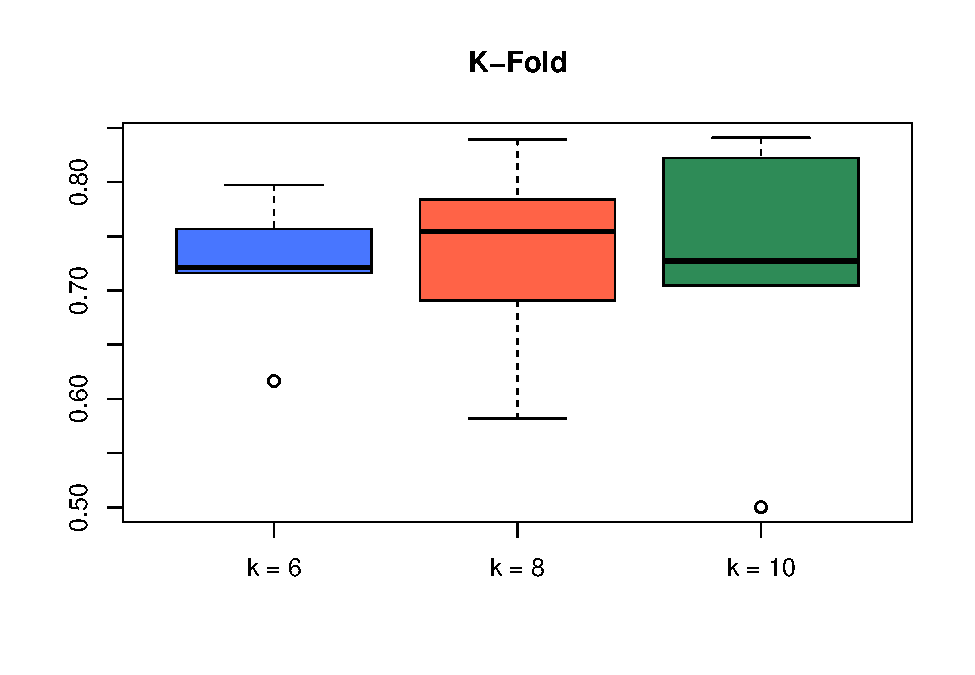
\includegraphics{TP3_MERR_HABBOU_KHIDOUR_files/figure-latex/unnamed-chunk-24-1} \end{center}

The principle behind K-Fold cross validation is that we start by
dividing our data set into K equal parts. Then we will train our model
on the K-1 first parts and use the last part to test the model. Then we
will use another combination of parts to train and test our model until
we computed all the possible combinations. In the end, every part of the
data set is used for testing and we can then have an idea of the
performance of our model on new data.

In our case we did 3 different K-Folds for K equal to 6, 8 and 10. By
looking at the boxplots we can see that the median of our accuracy is
around \(75\,\%\) with maximum and minimum values that can go from
\(60\,\%\) to \(80\,\%\) for the 10-fold.

\hypertarget{variable-selection}{%
\section{Variable Selection}\label{variable-selection}}

\hypertarget{statistical-approach}{%
\subsection{Statistical Approach}\label{statistical-approach}}

We start by setting up a model with all the variables and another with
only an intercept:

\begin{Shaded}
\begin{Highlighting}[]
\NormalTok{reg\_all }\OtherTok{\textless{}{-}} \FunctionTok{glm}\NormalTok{(YBin }\SpecialCharTok{\textasciitilde{}}\NormalTok{., }\AttributeTok{data =}\NormalTok{ diabetes\_data, }\AttributeTok{family =}\NormalTok{ binomial)}
\NormalTok{reg\_none }\OtherTok{\textless{}{-}} \FunctionTok{glm}\NormalTok{(YBin }\SpecialCharTok{\textasciitilde{}} \DecValTok{1}\NormalTok{, }\AttributeTok{data =}\NormalTok{ diabetes\_data, }\AttributeTok{family =}\NormalTok{ binomial)}
\end{Highlighting}
\end{Shaded}

\hypertarget{forward-logistic-regression}{%
\subsubsection{Forward Logistic
Regression}\label{forward-logistic-regression}}

\begin{Shaded}
\begin{Highlighting}[]
\NormalTok{reg\_forward }\OtherTok{\textless{}{-}} \FunctionTok{step}\NormalTok{(reg\_none, }\FunctionTok{list}\NormalTok{(}\AttributeTok{upper =}\NormalTok{ reg\_all), }\AttributeTok{direction =} \StringTok{\textquotesingle{}forward\textquotesingle{}}\NormalTok{)}
\end{Highlighting}
\end{Shaded}

\begin{verbatim}
Start:  AIC=614.74
YBin ~ 1

       Df Deviance    AIC
+ S5    1   500.61 504.61
+ BMI   1   507.06 511.06
+ BP    1   549.95 553.95
+ S4    1   552.60 556.60
+ S3    1   555.06 559.06
+ S6    1   573.71 577.71
+ S1    1   601.14 605.14
+ AGE   1   601.63 605.63
+ S2    1   604.41 608.41
<none>      612.74 614.74
+ SEX   1   612.73 616.73

Step:  AIC=504.61
YBin ~ S5

       Df Deviance    AIC
+ BMI   1   457.80 463.80
+ BP    1   480.20 486.20
+ S3    1   485.31 491.31
+ S1    1   494.40 500.40
+ SEX   1   497.09 503.09
+ S6    1   497.33 503.33
+ S4    1   497.75 503.75
<none>      500.61 504.61
+ S2    1   499.98 505.98
+ AGE   1   500.18 506.18

Step:  AIC=463.8
YBin ~ S5 + BMI

       Df Deviance    AIC
+ BP    1   448.52 456.52
+ S1    1   449.40 457.40
+ S3    1   450.90 458.90
+ SEX   1   454.15 462.15
+ S2    1   454.55 462.55
<none>      457.80 463.80
+ S4    1   457.56 465.56
+ S6    1   457.56 465.56
+ AGE   1   457.78 465.78

Step:  AIC=456.52
YBin ~ S5 + BMI + BP

       Df Deviance    AIC
+ S1    1   438.95 448.95
+ S3    1   440.93 450.93
+ SEX   1   441.96 451.96
+ S2    1   444.62 454.62
<none>      448.52 456.52
+ AGE   1   448.10 458.10
+ S4    1   448.24 458.24
+ S6    1   448.48 458.48

Step:  AIC=448.95
YBin ~ S5 + BMI + BP + S1

       Df Deviance    AIC
+ SEX   1   431.06 443.06
+ S2    1   434.89 446.89
+ S3    1   435.61 447.61
+ S4    1   436.32 448.32
<none>      438.95 448.95
+ AGE   1   438.91 450.91
+ S6    1   438.94 450.94

Step:  AIC=443.06
YBin ~ S5 + BMI + BP + S1 + SEX

       Df Deviance    AIC
+ S2    1   419.13 433.13
+ S3    1   420.41 434.41
+ S4    1   422.48 436.48
<none>      431.06 443.06
+ S6    1   430.85 444.85
+ AGE   1   431.02 445.02

Step:  AIC=433.13
YBin ~ S5 + BMI + BP + S1 + SEX + S2

       Df Deviance    AIC
<none>      419.13 433.13
+ AGE   1   419.00 435.00
+ S4    1   419.12 435.12
+ S3    1   419.12 435.12
+ S6    1   419.13 435.13
\end{verbatim}

We can observe that the forward logistic regression give us a model
which contains the following variables: \(S5\), \(BMI\), \(BP\), \(S1\),
\(SEX\) and \(S5\) with an AIC equal to \(433\).

\hypertarget{backward-logistic-regression}{%
\subsubsection{Backward Logistic
Regression}\label{backward-logistic-regression}}

\begin{Shaded}
\begin{Highlighting}[]
\NormalTok{reg\_back }\OtherTok{\textless{}{-}} \FunctionTok{step}\NormalTok{(reg\_all, }\AttributeTok{direction =} \StringTok{\textquotesingle{}backward\textquotesingle{}}\NormalTok{)}
\end{Highlighting}
\end{Shaded}

\begin{verbatim}
Start:  AIC=440.97
YBin ~ AGE + SEX + BMI + BP + S1 + S2 + S3 + S4 + S5 + S6

       Df Deviance    AIC
- S6    1   418.97 438.97
- S3    1   418.97 438.97
- S4    1   418.98 438.98
- AGE   1   419.11 439.11
- S2    1   420.19 440.19
- S1    1   420.79 440.79
<none>      418.97 440.97
- S5    1   427.77 447.77
- BP    1   433.51 453.51
- SEX   1   434.72 454.72
- BMI   1   437.80 457.80

Step:  AIC=438.97
YBin ~ AGE + SEX + BMI + BP + S1 + S2 + S3 + S4 + S5

       Df Deviance    AIC
- S3    1   418.97 436.97
- S4    1   418.98 436.98
- AGE   1   419.12 437.12
- S2    1   420.20 438.20
- S1    1   420.80 438.80
<none>      418.97 438.97
- S5    1   427.88 445.88
- BP    1   434.04 452.04
- SEX   1   434.76 452.76
- BMI   1   438.19 456.19

Step:  AIC=436.97
YBin ~ AGE + SEX + BMI + BP + S1 + S2 + S4 + S5

       Df Deviance    AIC
- S4    1   419.00 435.00
- AGE   1   419.12 435.12
<none>      418.97 436.97
- S2    1   422.28 438.28
- S1    1   427.40 443.40
- BP    1   434.05 450.05
- SEX   1   434.79 450.79
- BMI   1   438.29 454.29
- S5    1   441.41 457.41

Step:  AIC=435
YBin ~ AGE + SEX + BMI + BP + S1 + S2 + S5

       Df Deviance    AIC
- AGE   1   419.13 433.13
<none>      419.00 435.00
- S2    1   431.02 445.02
- BP    1   434.05 448.05
- SEX   1   434.83 448.83
- BMI   1   438.30 452.30
- S1    1   438.91 452.91
- S5    1   480.74 494.74

Step:  AIC=433.13
YBin ~ SEX + BMI + BP + S1 + S2 + S5

       Df Deviance    AIC
<none>      419.13 433.13
- S2    1   431.06 443.06
- SEX   1   434.89 446.89
- BP    1   435.39 447.39
- BMI   1   438.47 450.47
- S1    1   438.92 450.92
- S5    1   480.94 492.94
\end{verbatim}

We can observe that the backward logistic regression give us a model
which contains the following variables: \(S5\), \(BMI\), \(BP\), \(S1\),
\(SEX\) and \(S5\) with an AIC equal to \(433\).

\hypertarget{stepwise-logistic-regression}{%
\subsubsection{Stepwise Logistic
Regression}\label{stepwise-logistic-regression}}

\begin{Shaded}
\begin{Highlighting}[]
\NormalTok{reg\_both }\OtherTok{\textless{}{-}} \FunctionTok{step}\NormalTok{(reg\_all, }\AttributeTok{direction =} \StringTok{\textquotesingle{}both\textquotesingle{}}\NormalTok{)}
\end{Highlighting}
\end{Shaded}

\begin{verbatim}
Start:  AIC=440.97
YBin ~ AGE + SEX + BMI + BP + S1 + S2 + S3 + S4 + S5 + S6

       Df Deviance    AIC
- S6    1   418.97 438.97
- S3    1   418.97 438.97
- S4    1   418.98 438.98
- AGE   1   419.11 439.11
- S2    1   420.19 440.19
- S1    1   420.79 440.79
<none>      418.97 440.97
- S5    1   427.77 447.77
- BP    1   433.51 453.51
- SEX   1   434.72 454.72
- BMI   1   437.80 457.80

Step:  AIC=438.97
YBin ~ AGE + SEX + BMI + BP + S1 + S2 + S3 + S4 + S5

       Df Deviance    AIC
- S3    1   418.97 436.97
- S4    1   418.98 436.98
- AGE   1   419.12 437.12
- S2    1   420.20 438.20
- S1    1   420.80 438.80
<none>      418.97 438.97
+ S6    1   418.97 440.97
- S5    1   427.88 445.88
- BP    1   434.04 452.04
- SEX   1   434.76 452.76
- BMI   1   438.19 456.19

Step:  AIC=436.97
YBin ~ AGE + SEX + BMI + BP + S1 + S2 + S4 + S5

       Df Deviance    AIC
- S4    1   419.00 435.00
- AGE   1   419.12 435.12
<none>      418.97 436.97
- S2    1   422.28 438.28
+ S3    1   418.97 438.97
+ S6    1   418.97 438.97
- S1    1   427.40 443.40
- BP    1   434.05 450.05
- SEX   1   434.79 450.79
- BMI   1   438.29 454.29
- S5    1   441.41 457.41

Step:  AIC=435
YBin ~ AGE + SEX + BMI + BP + S1 + S2 + S5

       Df Deviance    AIC
- AGE   1   419.13 433.13
<none>      419.00 435.00
+ S4    1   418.97 436.97
+ S3    1   418.98 436.98
+ S6    1   419.00 437.00
- S2    1   431.02 445.02
- BP    1   434.05 448.05
- SEX   1   434.83 448.83
- BMI   1   438.30 452.30
- S1    1   438.91 452.91
- S5    1   480.74 494.74

Step:  AIC=433.13
YBin ~ SEX + BMI + BP + S1 + S2 + S5

       Df Deviance    AIC
<none>      419.13 433.13
+ AGE   1   419.00 435.00
+ S4    1   419.12 435.12
+ S3    1   419.12 435.12
+ S6    1   419.13 435.13
- S2    1   431.06 443.06
- SEX   1   434.89 446.89
- BP    1   435.39 447.39
- BMI   1   438.47 450.47
- S1    1   438.92 450.92
- S5    1   480.94 492.94
\end{verbatim}

We can observe that the stepwise logistic regression give us a model
which contains the following variables: \(S5\), \(BMI\), \(BP\), \(S1\),
\(SEX\) and \(S5\) with an AIC equal to \(433\).

\hypertarget{final-model}{%
\subsubsection{Final model}\label{final-model}}

Each time, we obtain the same value for the \(AIC\) criteria which
equals \(433\). We could choose another criteria for our model
selection, such as \(BIC\) or \(C_p\). It could influence our model
because the formula we will minimize changes. This formula will depend
differently on the number of co-variables \(p\). So the choice of
criteria will always depend on the business constraint behind. More than
that, we can customize our criteria as we want by choosing the value of
\(\lambda\) in the function \(step\).

Our final model will be the following:

\begin{Shaded}
\begin{Highlighting}[]
\NormalTok{diabetes\_reg }\OtherTok{\textless{}{-}} \FunctionTok{lm}\NormalTok{(}\FunctionTok{formula}\NormalTok{(reg\_both), }\AttributeTok{data =}\NormalTok{ diabetes\_data)}
\FunctionTok{summary}\NormalTok{(diabetes\_reg)}
\end{Highlighting}
\end{Shaded}

\begin{verbatim}

Call:
lm(formula = formula(reg_both), data = diabetes_data)

Residuals:
     Min       1Q   Median       3Q      Max 
-1.02548 -0.29301 -0.00166  0.31694  0.94958 

Coefficients:
             Estimate Std. Error t value Pr(>|t|)    
(Intercept) -1.962754   0.188818 -10.395  < 2e-16 ***
SEX         -0.169907   0.042440  -4.003 7.34e-05 ***
BMI          0.024674   0.005261   4.690 3.66e-06 ***
BP           0.006835   0.001605   4.257 2.54e-05 ***
S1          -0.007748   0.001642  -4.719 3.20e-06 ***
S2           0.006534   0.001709   3.823 0.000151 ***
S5           0.457993   0.054360   8.425 5.31e-16 ***
---
Signif. codes:  0 '***' 0.001 '**' 0.01 '*' 0.05 '.' 0.1 ' ' 1

Residual standard error: 0.4021 on 435 degrees of freedom
Multiple R-squared:  0.3634,    Adjusted R-squared:  0.3546 
F-statistic: 41.38 on 6 and 435 DF,  p-value: < 2.2e-16
\end{verbatim}

From the summary of our regression we can tell that:

\begin{itemize}
\tightlist
\item
  The residuals are quite symmetrically distributed around their median;
\item
  The intercept is equal to \(-1.962754\), we also notice the influence
  of each co-variable on Y;
\item
  The standard error and the t-value are provided to show how the
  p-values were calculated;
\item
  ALL the p-values are very low which means that all co-variables are
  significant;
\item
  The \(R^2\) tells us that the p co-variables can explain \(36\,\%\) of
  the variation in the target variable YBin;
\item
  The first degree of freedom corresponds to \(p - 1\) with \(p = 7\)
  the number of variables of the model;
\item
  The second degree of freedom corresponds to \(n - p\) with \(n = 442\)
  the number of data points;
\end{itemize}

\hypertarget{penalized-methods}{%
\subsection{Penalized Methods}\label{penalized-methods}}

\begin{Shaded}
\begin{Highlighting}[]
\NormalTok{sample }\OtherTok{\textless{}{-}} \FunctionTok{sample}\NormalTok{(}\FunctionTok{c}\NormalTok{(}\ConstantTok{TRUE}\NormalTok{, }\ConstantTok{FALSE}\NormalTok{), }\FunctionTok{nrow}\NormalTok{(diabetes\_data), }\AttributeTok{replace =} \ConstantTok{TRUE}\NormalTok{, }\AttributeTok{prob =} \FunctionTok{c}\NormalTok{(}\FloatTok{0.8}\NormalTok{, }\FloatTok{0.2}\NormalTok{))}
\NormalTok{train\_data }\OtherTok{\textless{}{-}}\NormalTok{ diabetes\_data[sample, ]}
\NormalTok{test\_data }\OtherTok{\textless{}{-}}\NormalTok{ diabetes\_data[}\SpecialCharTok{!}\NormalTok{sample, ]}
\end{Highlighting}
\end{Shaded}

\hypertarget{ridge-regression}{%
\subsubsection{Ridge Regression}\label{ridge-regression}}

\hypertarget{regularization-path}{%
\paragraph{Regularization Path}\label{regularization-path}}

\begin{Shaded}
\begin{Highlighting}[]
\NormalTok{ridge }\OtherTok{\textless{}{-}} \FunctionTok{glmnet}\NormalTok{(}\AttributeTok{x =}\NormalTok{ train\_data[,}\SpecialCharTok{{-}}\DecValTok{11}\NormalTok{], }\AttributeTok{y =}\NormalTok{ train\_data}\SpecialCharTok{$}\NormalTok{YBin, }\AttributeTok{alpha =} \DecValTok{0}\NormalTok{, }\AttributeTok{family =} \StringTok{"binomial"}\NormalTok{)}
\FunctionTok{plot}\NormalTok{(ridge, }\AttributeTok{xvar =} \StringTok{"lambda"}\NormalTok{, }\AttributeTok{label =} \ConstantTok{TRUE}\NormalTok{, }\AttributeTok{lwd =} \DecValTok{2}\NormalTok{)}
\end{Highlighting}
\end{Shaded}

\begin{center}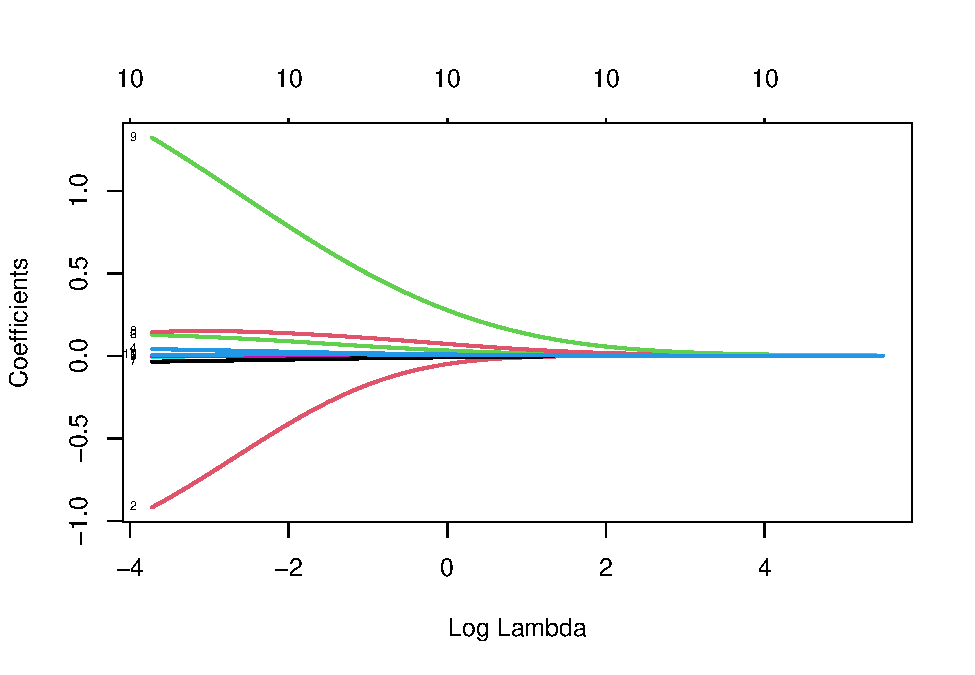
\includegraphics{TP3_MERR_HABBOU_KHIDOUR_files/figure-latex/unnamed-chunk-31-1} \end{center}

In the plot above, we can see the evolution of the coefficient values
depending on \(\lambda\) Knowing that we are doing a ridge regression,
we can tell that they will all converge to 0.

However, ridge regression does not perform feature selection and will
retain all available features in the final model. Therefore, a ridge
model is good if we suppose that there is a need to retain all features
in our model yet reduce the noise that less influential variables may
create.

If greater interpretation is necessary and many of the features are
redundant or irrelevant then a lasso or elastic net penalty may be
preferable.

\hypertarget{cross-validation}{%
\paragraph{Cross-Validation}\label{cross-validation}}

\begin{Shaded}
\begin{Highlighting}[]
\NormalTok{cv\_ridge }\OtherTok{\textless{}{-}} \FunctionTok{cv.glmnet}\NormalTok{(}\FunctionTok{as.matrix}\NormalTok{(train\_data[,}\SpecialCharTok{{-}}\DecValTok{11}\NormalTok{]), train\_data}\SpecialCharTok{$}\NormalTok{YBin, }
                      \AttributeTok{family =} \StringTok{"binomial"}\NormalTok{, }\AttributeTok{alpha =} \DecValTok{0}\NormalTok{, }\AttributeTok{type.measure =} \StringTok{"mse"}\NormalTok{)}
\FunctionTok{plot}\NormalTok{(cv\_ridge)}
\end{Highlighting}
\end{Shaded}

\begin{center}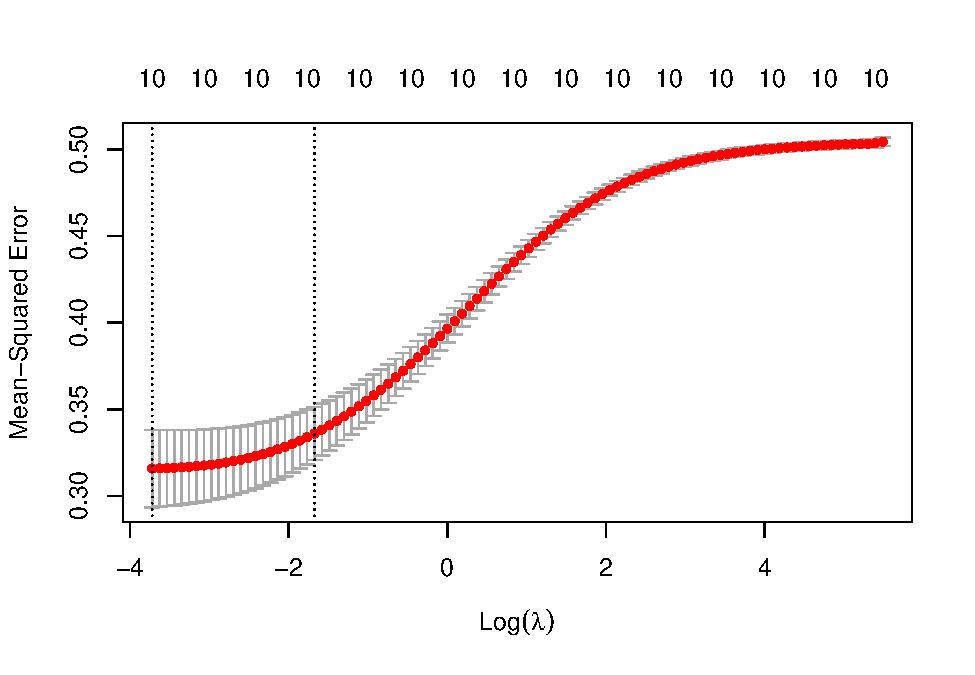
\includegraphics{TP3_MERR_HABBOU_KHIDOUR_files/figure-latex/unnamed-chunk-32-1} \end{center}

In the above plot, we visualize the cross validation curve:

\begin{itemize}
\item
  \(\lambda_{min}\) is the value which minimizes the Mean Squared Error
  in Cross-Validation;
\item
  \(\lambda_{1se}\) is the value which is the largest \(\lambda\) value
  within 1 standard error;
\item
  The intervals estimate variance of the loss metric (red points) they
  are computed using Cross-Validation;
\item
  The vertical lines show the locations of \(\lambda_{min}\) and
  \(\lambda_{1se}\);
\item
  The numbers across the top are the number of non-zero coefficients.
\end{itemize}

We observe a slight improvement in the Mean Squared Error as our penalty
\(log(\lambda)\) gets larger, suggesting that a regular OLS model likely
overfits the training data. But as we constrain it further by continuing
to increase the penalty our Mean Squared Error starts to increase.

\hypertarget{lambda-min}{%
\paragraph{Lambda Min}\label{lambda-min}}

\begin{Shaded}
\begin{Highlighting}[]
\NormalTok{lambda\_min }\OtherTok{\textless{}{-}}\NormalTok{ cv\_ridge}\SpecialCharTok{$}\NormalTok{lambda.min}
\NormalTok{ridge\_min }\OtherTok{\textless{}{-}} \FunctionTok{glmnet}\NormalTok{(}\AttributeTok{x =}\NormalTok{ train\_data[,}\SpecialCharTok{{-}}\DecValTok{11}\NormalTok{], }\AttributeTok{y =}\NormalTok{ train\_data}\SpecialCharTok{$}\NormalTok{YBin, }
                    \AttributeTok{alpha =} \DecValTok{0}\NormalTok{, }\AttributeTok{family =} \StringTok{"binomial"}\NormalTok{, }\AttributeTok{lambda =}\NormalTok{ lambda\_min)}
\NormalTok{ridge\_min}\SpecialCharTok{$}\NormalTok{beta}
\end{Highlighting}
\end{Shaded}

\begin{verbatim}
10 x 1 sparse Matrix of class "dgCMatrix"
               s0
AGE -0.0006809721
SEX -0.9178811616
BMI  0.1267419368
BP   0.0408932726
S1  -0.0045648736
S2  -0.0032411765
S3  -0.0353723178
S4   0.1433731000
S5   1.3227681473
S6   0.0059168421
\end{verbatim}

The model obtained using \(\lambda_{min}\) gives us the model with
lowest Mean Squared Error, which can seem to be a good choice but in
fact it can implies overfitting.

\begin{Shaded}
\begin{Highlighting}[]
\NormalTok{prediction\_min }\OtherTok{\textless{}{-}} \FunctionTok{as.numeric}\NormalTok{(}\FunctionTok{predict}\NormalTok{(ridge\_min, }\FunctionTok{as.matrix}\NormalTok{(diabetes\_data[,}\SpecialCharTok{{-}}\DecValTok{11}\NormalTok{]), }\AttributeTok{type =} \StringTok{"response"}\NormalTok{) }\SpecialCharTok{\textgreater{}} \FloatTok{0.5}\NormalTok{)}
\end{Highlighting}
\end{Shaded}

Using the Maximum A Posteriori criteria we can make predictions for our
binary variable \(YBin\):

\begin{Shaded}
\begin{Highlighting}[]
\FunctionTok{table}\NormalTok{(prediction\_min)}
\end{Highlighting}
\end{Shaded}

\begin{verbatim}
prediction_min
  0   1 
216 226 
\end{verbatim}

Knowing that our target variable have the following values:

\begin{Shaded}
\begin{Highlighting}[]
\FunctionTok{table}\NormalTok{(diabetes\_data}\SpecialCharTok{$}\NormalTok{YBin)}
\end{Highlighting}
\end{Shaded}

\begin{verbatim}

  0   1 
221 221 
\end{verbatim}

By comparing the both tables we can tell that our predictions are quite
consistent, since our model has nearly the same count for 0 and 1 than
the target variable in our data set.

\hypertarget{confusion-matrix-1}{%
\paragraph{Confusion Matrix}\label{confusion-matrix-1}}

\begin{Shaded}
\begin{Highlighting}[]
\NormalTok{confusion\_matrix }\OtherTok{\textless{}{-}} \FunctionTok{table}\NormalTok{(diabetes\_data}\SpecialCharTok{$}\NormalTok{YBin, prediction\_min)}
\NormalTok{confusion\_matrix}
\end{Highlighting}
\end{Shaded}

\begin{verbatim}
   prediction_min
      0   1
  0 165  56
  1  51 170
\end{verbatim}

\hypertarget{accuracy-1}{%
\paragraph{Accuracy}\label{accuracy-1}}

\begin{Shaded}
\begin{Highlighting}[]
\NormalTok{accuracy }\OtherTok{\textless{}{-}}\NormalTok{ (confusion\_matrix[}\DecValTok{1}\NormalTok{,}\DecValTok{1}\NormalTok{] }\SpecialCharTok{+}\NormalTok{ confusion\_matrix[}\DecValTok{2}\NormalTok{,}\DecValTok{2}\NormalTok{]) }\SpecialCharTok{/} \FunctionTok{nrow}\NormalTok{(diabetes\_data)}
\NormalTok{accuracy}
\end{Highlighting}
\end{Shaded}

\begin{verbatim}
[1] 0.7579186
\end{verbatim}

The accuracy is equal to \(76.2\,\%\).

\hypertarget{lambda-1se}{%
\paragraph{Lambda 1se}\label{lambda-1se}}

\begin{Shaded}
\begin{Highlighting}[]
\NormalTok{lambda\_1se }\OtherTok{\textless{}{-}}\NormalTok{ cv\_ridge}\SpecialCharTok{$}\NormalTok{lambda}\FloatTok{.1}\NormalTok{se}
\NormalTok{ridge\_1se }\OtherTok{\textless{}{-}} \FunctionTok{glmnet}\NormalTok{(}\AttributeTok{x =}\NormalTok{ train\_data[,}\SpecialCharTok{{-}}\DecValTok{11}\NormalTok{], }\AttributeTok{y =}\NormalTok{ train\_data}\SpecialCharTok{$}\NormalTok{YBin, }
                    \AttributeTok{alpha =} \DecValTok{0}\NormalTok{, }\AttributeTok{family =} \StringTok{"binomial"}\NormalTok{, }\AttributeTok{lambda =}\NormalTok{ lambda\_1se)}
\NormalTok{ridge\_1se}\SpecialCharTok{$}\NormalTok{beta}
\end{Highlighting}
\end{Shaded}

\begin{verbatim}
10 x 1 sparse Matrix of class "dgCMatrix"
               s0
AGE  0.0011417634
SEX -0.3232491500
BMI  0.0784986834
BP   0.0216252031
S1  -0.0005624766
S2  -0.0014677354
S3  -0.0197188152
S4   0.1288575949
S5   0.6848891539
S6   0.0093567340
\end{verbatim}

The model obtained using \(\lambda_{1se}\) gives us a simpler model
which can avoid overfitting.

\begin{Shaded}
\begin{Highlighting}[]
\NormalTok{prediction\_1se }\OtherTok{\textless{}{-}} \FunctionTok{as.numeric}\NormalTok{(}\FunctionTok{predict}\NormalTok{(ridge\_1se, }\FunctionTok{as.matrix}\NormalTok{(diabetes\_data[,}\SpecialCharTok{{-}}\DecValTok{11}\NormalTok{]), }\AttributeTok{type =} \StringTok{"response"}\NormalTok{) }\SpecialCharTok{\textgreater{}} \FloatTok{0.5}\NormalTok{)}
\end{Highlighting}
\end{Shaded}

Using the Maximum A Posteriori criteria we can make predictions for our
binary variable \(YBin\):

\begin{Shaded}
\begin{Highlighting}[]
\FunctionTok{table}\NormalTok{(prediction\_1se)}
\end{Highlighting}
\end{Shaded}

\begin{verbatim}
prediction_1se
  0   1 
213 229 
\end{verbatim}

Knowing that our target variable have the following values:

\begin{Shaded}
\begin{Highlighting}[]
\FunctionTok{table}\NormalTok{(diabetes\_data}\SpecialCharTok{$}\NormalTok{YBin)}
\end{Highlighting}
\end{Shaded}

\begin{verbatim}

  0   1 
221 221 
\end{verbatim}

By comparing the both tables we can tell that our predictions are quite
consistent, since our model has nearly the same count for 0 and 1 than
the target variable in our data set.

\hypertarget{confusion-matrix-2}{%
\paragraph{Confusion Matrix}\label{confusion-matrix-2}}

\begin{Shaded}
\begin{Highlighting}[]
\NormalTok{confusion\_matrix }\OtherTok{\textless{}{-}} \FunctionTok{table}\NormalTok{(diabetes\_data}\SpecialCharTok{$}\NormalTok{YBin, prediction\_1se)}
\NormalTok{confusion\_matrix}
\end{Highlighting}
\end{Shaded}

\begin{verbatim}
   prediction_1se
      0   1
  0 166  55
  1  47 174
\end{verbatim}

\hypertarget{accuracy-2}{%
\paragraph{Accuracy}\label{accuracy-2}}

\begin{Shaded}
\begin{Highlighting}[]
\NormalTok{accuracy }\OtherTok{\textless{}{-}}\NormalTok{ (confusion\_matrix[}\DecValTok{1}\NormalTok{,}\DecValTok{1}\NormalTok{] }\SpecialCharTok{+}\NormalTok{ confusion\_matrix[}\DecValTok{2}\NormalTok{,}\DecValTok{2}\NormalTok{]) }\SpecialCharTok{/} \FunctionTok{nrow}\NormalTok{(diabetes\_data)}
\NormalTok{accuracy}
\end{Highlighting}
\end{Shaded}

\begin{verbatim}
[1] 0.7692308
\end{verbatim}

The accuracy is equal to \(76.6\,\%\).

\hypertarget{fold}{%
\paragraph{10-Fold}\label{fold}}

\begin{Shaded}
\begin{Highlighting}[]
\NormalTok{kfold\_ridge }\OtherTok{\textless{}{-}} \ControlFlowTok{function}\NormalTok{(k, lambda)}
\NormalTok{\{}
  \CommentTok{\# create a vector of length number of folds}
\NormalTok{  performance }\OtherTok{\textless{}{-}} \FunctionTok{vector}\NormalTok{(}\AttributeTok{length =}\NormalTok{ k)}
  \CommentTok{\# create a sequence from 1 to k}
\NormalTok{  folds }\OtherTok{\textless{}{-}} \FunctionTok{cut}\NormalTok{(}\FunctionTok{seq}\NormalTok{(}\DecValTok{1}\NormalTok{,}\FunctionTok{nrow}\NormalTok{(diabetes\_data)), }\AttributeTok{breaks =}\NormalTok{ k, }\AttributeTok{labels =} \ConstantTok{FALSE}\NormalTok{)}
  \CommentTok{\# perform 10 fold cross validation}
  \ControlFlowTok{for}\NormalTok{(i }\ControlFlowTok{in} \DecValTok{1}\SpecialCharTok{:}\NormalTok{k)}
\NormalTok{  \{}
    \CommentTok{\# split data by fold}
\NormalTok{    index }\OtherTok{\textless{}{-}} \FunctionTok{which}\NormalTok{(folds }\SpecialCharTok{==}\NormalTok{ i, }\AttributeTok{arr.ind =} \ConstantTok{TRUE}\NormalTok{)}
\NormalTok{    test\_data }\OtherTok{\textless{}{-}}\NormalTok{ diabetes\_data[index,]}
\NormalTok{    train\_data }\OtherTok{\textless{}{-}}\NormalTok{ diabetes\_data[}\SpecialCharTok{{-}}\NormalTok{index,]}
    \CommentTok{\# train the logistic regression on the train data set}
\NormalTok{    reg\_log }\OtherTok{\textless{}{-}} \FunctionTok{glmnet}\NormalTok{(}\AttributeTok{x =}\NormalTok{ train\_data[,}\SpecialCharTok{{-}}\DecValTok{11}\NormalTok{], }\AttributeTok{y =}\NormalTok{ train\_data}\SpecialCharTok{$}\NormalTok{YBin, }
                      \AttributeTok{alpha =} \DecValTok{0}\NormalTok{, }\AttributeTok{family =} \StringTok{"binomial"}\NormalTok{, }\AttributeTok{lambda =}\NormalTok{ lambda)}
    \CommentTok{\# make predictions}
\NormalTok{    prediction }\OtherTok{\textless{}{-}} \FunctionTok{as.numeric}\NormalTok{(}\FunctionTok{predict}\NormalTok{(reg\_log, }\FunctionTok{as.matrix}\NormalTok{(test\_data[,}\SpecialCharTok{{-}}\DecValTok{11}\NormalTok{]), }\AttributeTok{type =} \StringTok{"response"}\NormalTok{) }\SpecialCharTok{\textgreater{}} \FloatTok{0.5}\NormalTok{)}
\NormalTok{    confusion\_matrix }\OtherTok{\textless{}{-}} \FunctionTok{table}\NormalTok{(prediction, test\_data}\SpecialCharTok{$}\NormalTok{YBin)}
    \CommentTok{\# compute the performance}
\NormalTok{    performance[i] }\OtherTok{\textless{}{-}}\NormalTok{ (confusion\_matrix[}\DecValTok{1}\NormalTok{,}\DecValTok{1}\NormalTok{] }\SpecialCharTok{+}\NormalTok{ confusion\_matrix[}\DecValTok{2}\NormalTok{,}\DecValTok{2}\NormalTok{]) }\SpecialCharTok{/} \FunctionTok{nrow}\NormalTok{(test\_data)}
\NormalTok{  \} }
  \FunctionTok{return}\NormalTok{ (performance)}
\NormalTok{\}}
\end{Highlighting}
\end{Shaded}

\begin{Shaded}
\begin{Highlighting}[]
\FunctionTok{boxplot}\NormalTok{(}\FunctionTok{kfold\_ridge}\NormalTok{(}\DecValTok{10}\NormalTok{, lambda\_min), }\FunctionTok{kfold\_ridge}\NormalTok{(}\DecValTok{10}\NormalTok{, lambda\_1se), }\AttributeTok{main =} \StringTok{"K{-}Fold"}\NormalTok{, }
        \AttributeTok{names =} \FunctionTok{c}\NormalTok{(}\StringTok{"lambda\_min"}\NormalTok{, }\StringTok{"lambda\_1se"}\NormalTok{), }\AttributeTok{col =} \FunctionTok{c}\NormalTok{(}\StringTok{"royalblue1"}\NormalTok{, }\StringTok{"tomato1"}\NormalTok{))}
\end{Highlighting}
\end{Shaded}

\begin{center}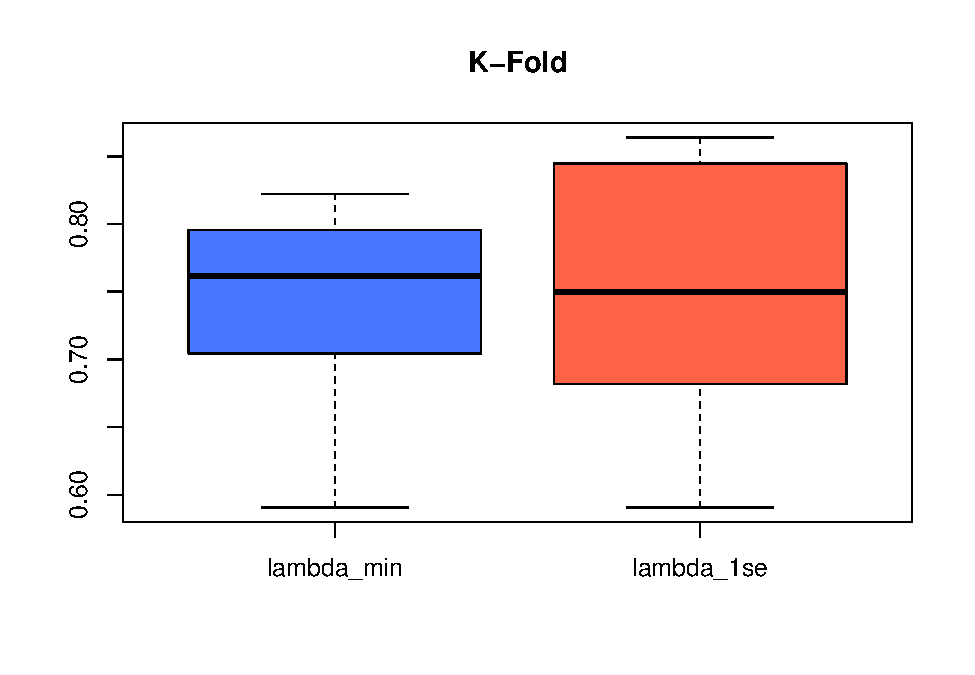
\includegraphics{TP3_MERR_HABBOU_KHIDOUR_files/figure-latex/unnamed-chunk-46-1} \end{center}

In our case we did two 10-Folds with \(\lambda_{min}\) and
\(\lambda_{1se}\). By looking at the boxplots we can see that the median
of our accuracy in between \(75\,\%\) and \(80\,\%\) for the two models.
But we can clearly observe that the box for \(\lambda_{1se}\) is higher
than the one for \(\lambda_{min}\) which means in generally we will have
a better accuracy by using \(\lambda_{1se}\). More than that, we know
that with \(\lambda_{1se}\) we are having a larger penalization than
with \(\lambda_{min}\) which explains why we have a larger interquartile
range and a larger distance between the minmum and the maximum.

\hypertarget{lasso-regression}{%
\subsubsection{Lasso Regression}\label{lasso-regression}}

\hypertarget{regularization-path-1}{%
\paragraph{Regularization Path}\label{regularization-path-1}}

\begin{Shaded}
\begin{Highlighting}[]
\NormalTok{lasso }\OtherTok{\textless{}{-}} \FunctionTok{glmnet}\NormalTok{(}\AttributeTok{x =}\NormalTok{ train\_data[,}\SpecialCharTok{{-}}\DecValTok{11}\NormalTok{], }\AttributeTok{y =}\NormalTok{ train\_data}\SpecialCharTok{$}\NormalTok{YBin, }\AttributeTok{alpha =} \DecValTok{1}\NormalTok{, }\AttributeTok{family =} \StringTok{"binomial"}\NormalTok{)}
\FunctionTok{plot}\NormalTok{(lasso, }\AttributeTok{xvar =} \StringTok{"lambda"}\NormalTok{, }\AttributeTok{label =} \ConstantTok{TRUE}\NormalTok{, }\AttributeTok{lwd =} \DecValTok{2}\NormalTok{)}
\end{Highlighting}
\end{Shaded}

\begin{center}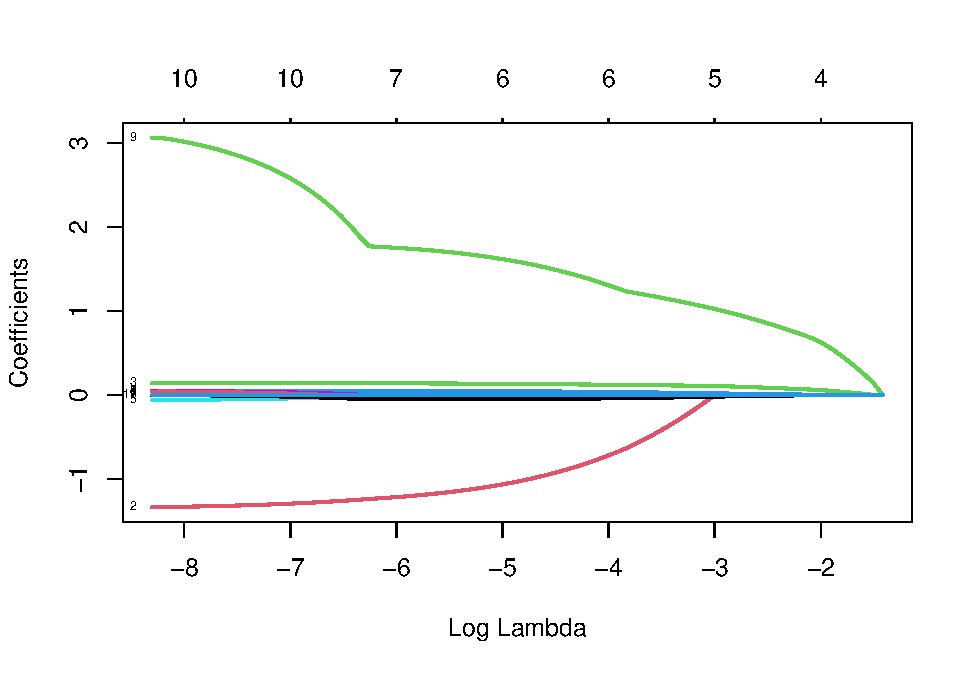
\includegraphics{TP3_MERR_HABBOU_KHIDOUR_files/figure-latex/unnamed-chunk-47-1} \end{center}

In the plot above, we can see the evolution of the coefficient values
depending on \(\lambda\) Knowing that we are doing a lasso regression,
we can tell that they will all converge to 0 one by one and not all at
the same time.

When a data set has many co-variables, lasso can be used to identify and
extract those co-variables which are the most significant. Switching to
the lasso penalty also conducts automated variable selection.

\hypertarget{cross-validation-1}{%
\paragraph{Cross-Validation}\label{cross-validation-1}}

\begin{Shaded}
\begin{Highlighting}[]
\NormalTok{cv\_lasso }\OtherTok{\textless{}{-}} \FunctionTok{cv.glmnet}\NormalTok{(}\FunctionTok{as.matrix}\NormalTok{(train\_data[,}\SpecialCharTok{{-}}\DecValTok{11}\NormalTok{]), train\_data}\SpecialCharTok{$}\NormalTok{YBin, }
                      \AttributeTok{family =} \StringTok{"binomial"}\NormalTok{, }\AttributeTok{alpha =} \DecValTok{1}\NormalTok{, }\AttributeTok{type.measure =} \StringTok{"mse"}\NormalTok{)}
\FunctionTok{plot}\NormalTok{(cv\_lasso)}
\end{Highlighting}
\end{Shaded}

\begin{center}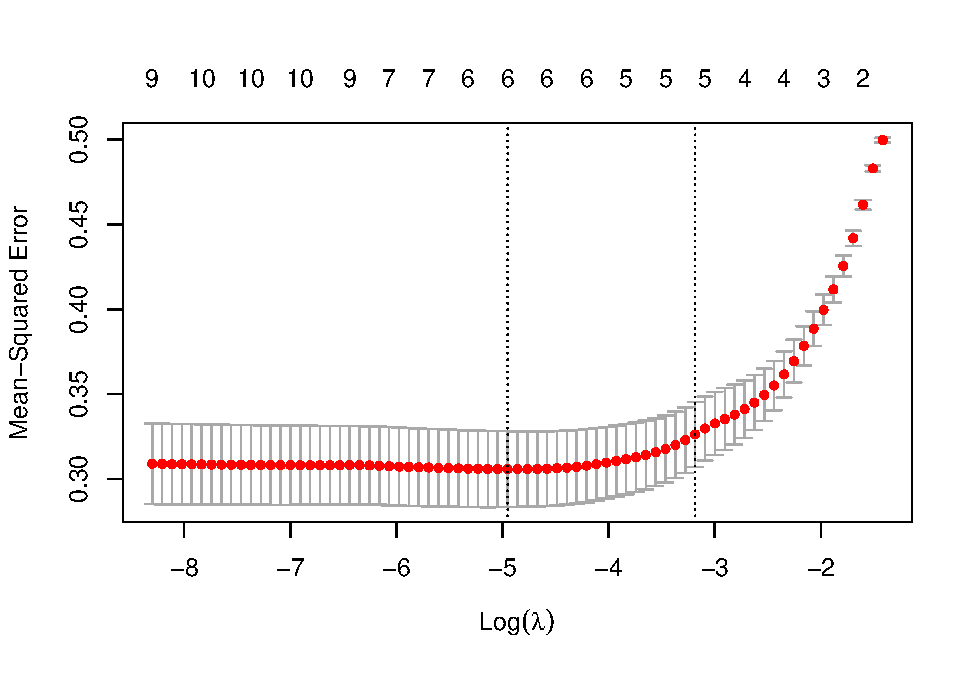
\includegraphics{TP3_MERR_HABBOU_KHIDOUR_files/figure-latex/unnamed-chunk-48-1} \end{center}

We observe a slight improvement in the Mean Squared Error as our penalty
\(log(\lambda)\) gets larger, suggesting that a regular OLS model likely
overfits the training data. But as we constrain it further by continuing
to increase the penalty our Mean Squared Error starts to increase.

\hypertarget{lambda-min-1}{%
\paragraph{Lambda Min}\label{lambda-min-1}}

\begin{Shaded}
\begin{Highlighting}[]
\NormalTok{lambda\_min }\OtherTok{\textless{}{-}}\NormalTok{ cv\_lasso}\SpecialCharTok{$}\NormalTok{lambda.min}
\NormalTok{lasso\_min }\OtherTok{\textless{}{-}} \FunctionTok{glmnet}\NormalTok{(}\AttributeTok{x =}\NormalTok{ train\_data[,}\SpecialCharTok{{-}}\DecValTok{11}\NormalTok{], }\AttributeTok{y =}\NormalTok{ train\_data}\SpecialCharTok{$}\NormalTok{YBin, }
                    \AttributeTok{alpha =} \DecValTok{1}\NormalTok{, }\AttributeTok{family =} \StringTok{"binomial"}\NormalTok{, }\AttributeTok{lambda =}\NormalTok{ lambda\_min)}
\NormalTok{lasso\_min}\SpecialCharTok{$}\NormalTok{beta}
\end{Highlighting}
\end{Shaded}

\begin{verbatim}
10 x 1 sparse Matrix of class "dgCMatrix"
             s0
AGE  .         
SEX -1.05241764
BMI  0.13366262
BP   0.04567162
S1  -0.00527105
S2   .         
S3  -0.04687441
S4   .         
S5   1.60762089
S6   .         
\end{verbatim}

The model obtained using \(\lambda_{min}\) gives us the model with
lowest Mean Squared Error, which can seem to be a good choice but in
fact it can implies overfitting. We observe that the model does not
contain \(AGE\), \(S2\) and \(S4\).

\begin{Shaded}
\begin{Highlighting}[]
\NormalTok{prediction\_min }\OtherTok{\textless{}{-}} \FunctionTok{as.numeric}\NormalTok{(}\FunctionTok{predict}\NormalTok{(lasso\_min, }\FunctionTok{as.matrix}\NormalTok{(diabetes\_data[,}\SpecialCharTok{{-}}\DecValTok{11}\NormalTok{]), }\AttributeTok{type =} \StringTok{"response"}\NormalTok{) }\SpecialCharTok{\textgreater{}} \FloatTok{0.5}\NormalTok{)}
\end{Highlighting}
\end{Shaded}

Using the Maximum A Posteriori criteria we can make predictions for our
binary variable \(YBin\):

\begin{Shaded}
\begin{Highlighting}[]
\FunctionTok{table}\NormalTok{(prediction\_min)}
\end{Highlighting}
\end{Shaded}

\begin{verbatim}
prediction_min
  0   1 
216 226 
\end{verbatim}

Knowing that our target variable have the following values:

\begin{Shaded}
\begin{Highlighting}[]
\FunctionTok{table}\NormalTok{(diabetes\_data}\SpecialCharTok{$}\NormalTok{YBin)}
\end{Highlighting}
\end{Shaded}

\begin{verbatim}

  0   1 
221 221 
\end{verbatim}

By comparing the both tables we can tell that our predictions are quite
consistent, since our model has nearly the same count for 0 and 1 than
the target variable in our data set.

\hypertarget{confusion-matrix-3}{%
\paragraph{Confusion Matrix}\label{confusion-matrix-3}}

\begin{Shaded}
\begin{Highlighting}[]
\NormalTok{confusion\_matrix }\OtherTok{\textless{}{-}} \FunctionTok{table}\NormalTok{(diabetes\_data}\SpecialCharTok{$}\NormalTok{YBin, prediction\_min)}
\NormalTok{confusion\_matrix}
\end{Highlighting}
\end{Shaded}

\begin{verbatim}
   prediction_min
      0   1
  0 164  57
  1  52 169
\end{verbatim}

\hypertarget{accuracy-3}{%
\paragraph{Accuracy}\label{accuracy-3}}

\begin{Shaded}
\begin{Highlighting}[]
\NormalTok{accuracy }\OtherTok{\textless{}{-}}\NormalTok{ (confusion\_matrix[}\DecValTok{1}\NormalTok{,}\DecValTok{1}\NormalTok{] }\SpecialCharTok{+}\NormalTok{ confusion\_matrix[}\DecValTok{2}\NormalTok{,}\DecValTok{2}\NormalTok{]) }\SpecialCharTok{/} \FunctionTok{nrow}\NormalTok{(diabetes\_data)}
\NormalTok{accuracy}
\end{Highlighting}
\end{Shaded}

\begin{verbatim}
[1] 0.7533937
\end{verbatim}

The accuracy is equal to \(76.5\,\%\).

\hypertarget{lambda-1se-1}{%
\paragraph{Lambda 1se}\label{lambda-1se-1}}

\begin{Shaded}
\begin{Highlighting}[]
\NormalTok{lambda\_1se }\OtherTok{\textless{}{-}}\NormalTok{ cv\_lasso}\SpecialCharTok{$}\NormalTok{lambda}\FloatTok{.1}\NormalTok{se}
\NormalTok{lasso\_1se }\OtherTok{\textless{}{-}} \FunctionTok{glmnet}\NormalTok{(}\AttributeTok{x =}\NormalTok{ train\_data[,}\SpecialCharTok{{-}}\DecValTok{11}\NormalTok{], }\AttributeTok{y =}\NormalTok{ train\_data}\SpecialCharTok{$}\NormalTok{YBin, }
                    \AttributeTok{alpha =} \DecValTok{1}\NormalTok{, }\AttributeTok{family =} \StringTok{"binomial"}\NormalTok{, }\AttributeTok{lambda =}\NormalTok{ lambda\_1se)}
\NormalTok{lasso\_1se}\SpecialCharTok{$}\NormalTok{beta}
\end{Highlighting}
\end{Shaded}

\begin{verbatim}
10 x 1 sparse Matrix of class "dgCMatrix"
             s0
AGE  .         
SEX -0.16687686
BMI  0.11145510
BP   0.02343538
S1   .         
S2   .         
S3  -0.02291438
S4   .         
S5   1.07652982
S6   .         
\end{verbatim}

The model obtained using \(\lambda_{1se}\) gives us a simpler model
which can avoid overfitting. We observe that the model does not contain
\(AGE\), \(S1\), \(S2\), \(S4\) and \(S6\), so the model is simpler than
the one with \(\lambda_{min}\).

\begin{Shaded}
\begin{Highlighting}[]
\NormalTok{prediction\_1se }\OtherTok{\textless{}{-}} \FunctionTok{as.numeric}\NormalTok{(}\FunctionTok{predict}\NormalTok{(lasso\_1se, }\FunctionTok{as.matrix}\NormalTok{(diabetes\_data[,}\SpecialCharTok{{-}}\DecValTok{11}\NormalTok{]), }\AttributeTok{type =} \StringTok{"response"}\NormalTok{) }\SpecialCharTok{\textgreater{}} \FloatTok{0.5}\NormalTok{)}
\end{Highlighting}
\end{Shaded}

Using the Maximum A Posteriori criteria we can make predictions for our
binary variable \(YBin\):

\begin{Shaded}
\begin{Highlighting}[]
\FunctionTok{table}\NormalTok{(prediction\_1se)}
\end{Highlighting}
\end{Shaded}

\begin{verbatim}
prediction_1se
  0   1 
215 227 
\end{verbatim}

Knowing that our target variable have the following values:

\begin{Shaded}
\begin{Highlighting}[]
\FunctionTok{table}\NormalTok{(diabetes\_data}\SpecialCharTok{$}\NormalTok{YBin)}
\end{Highlighting}
\end{Shaded}

\begin{verbatim}

  0   1 
221 221 
\end{verbatim}

By comparing the both tables we can tell that our predictions are quite
consistent, since our model has nearly the same count for 0 and 1 than
the target variable in our data set.

\hypertarget{confusion-matrix-4}{%
\paragraph{Confusion Matrix}\label{confusion-matrix-4}}

\begin{Shaded}
\begin{Highlighting}[]
\NormalTok{confusion\_matrix }\OtherTok{\textless{}{-}} \FunctionTok{table}\NormalTok{(diabetes\_data}\SpecialCharTok{$}\NormalTok{YBin, prediction\_1se)}
\NormalTok{confusion\_matrix}
\end{Highlighting}
\end{Shaded}

\begin{verbatim}
   prediction_1se
      0   1
  0 165  56
  1  50 171
\end{verbatim}

\hypertarget{accuracy-4}{%
\paragraph{Accuracy}\label{accuracy-4}}

\begin{Shaded}
\begin{Highlighting}[]
\NormalTok{accuracy }\OtherTok{\textless{}{-}}\NormalTok{ (confusion\_matrix[}\DecValTok{1}\NormalTok{,}\DecValTok{1}\NormalTok{] }\SpecialCharTok{+}\NormalTok{ confusion\_matrix[}\DecValTok{2}\NormalTok{,}\DecValTok{2}\NormalTok{]) }\SpecialCharTok{/} \FunctionTok{nrow}\NormalTok{(diabetes\_data)}
\NormalTok{accuracy}
\end{Highlighting}
\end{Shaded}

\begin{verbatim}
[1] 0.760181
\end{verbatim}

The accuracy is equal to \(74.8\,\%\).

\hypertarget{fold-1}{%
\paragraph{10-Fold}\label{fold-1}}

\begin{Shaded}
\begin{Highlighting}[]
\NormalTok{kfold\_lasso }\OtherTok{\textless{}{-}} \ControlFlowTok{function}\NormalTok{(k, lambda)}
\NormalTok{\{}
  \CommentTok{\# create a vector of length number of folds}
\NormalTok{  performance }\OtherTok{\textless{}{-}} \FunctionTok{vector}\NormalTok{(}\AttributeTok{length =}\NormalTok{ k)}
  \CommentTok{\# create a sequence from 1 to k}
\NormalTok{  folds }\OtherTok{\textless{}{-}} \FunctionTok{cut}\NormalTok{(}\FunctionTok{seq}\NormalTok{(}\DecValTok{1}\NormalTok{,}\FunctionTok{nrow}\NormalTok{(diabetes\_data)), }\AttributeTok{breaks =}\NormalTok{ k, }\AttributeTok{labels =} \ConstantTok{FALSE}\NormalTok{)}
  \CommentTok{\# perform 10 fold cross validation}
  \ControlFlowTok{for}\NormalTok{(i }\ControlFlowTok{in} \DecValTok{1}\SpecialCharTok{:}\NormalTok{k)}
\NormalTok{  \{}
    \CommentTok{\# split data by fold}
\NormalTok{    index }\OtherTok{\textless{}{-}} \FunctionTok{which}\NormalTok{(folds }\SpecialCharTok{==}\NormalTok{ i, }\AttributeTok{arr.ind =} \ConstantTok{TRUE}\NormalTok{)}
\NormalTok{    test\_data }\OtherTok{\textless{}{-}}\NormalTok{ diabetes\_data[index,]}
\NormalTok{    train\_data }\OtherTok{\textless{}{-}}\NormalTok{ diabetes\_data[}\SpecialCharTok{{-}}\NormalTok{index,]}
    \CommentTok{\# train the logistic regression on the train data set}
\NormalTok{    reg\_log }\OtherTok{\textless{}{-}} \FunctionTok{glmnet}\NormalTok{(}\AttributeTok{x =}\NormalTok{ train\_data[,}\SpecialCharTok{{-}}\DecValTok{11}\NormalTok{], }\AttributeTok{y =}\NormalTok{ train\_data}\SpecialCharTok{$}\NormalTok{YBin, }
                      \AttributeTok{alpha =} \DecValTok{1}\NormalTok{, }\AttributeTok{family =} \StringTok{"binomial"}\NormalTok{, }\AttributeTok{lambda =}\NormalTok{ lambda)}
    \CommentTok{\# make predictions}
\NormalTok{    prediction }\OtherTok{\textless{}{-}} \FunctionTok{as.numeric}\NormalTok{(}\FunctionTok{predict}\NormalTok{(reg\_log, }\FunctionTok{as.matrix}\NormalTok{(test\_data[,}\SpecialCharTok{{-}}\DecValTok{11}\NormalTok{]), }\AttributeTok{type =} \StringTok{"response"}\NormalTok{) }\SpecialCharTok{\textgreater{}} \FloatTok{0.5}\NormalTok{)}
\NormalTok{    confusion\_matrix }\OtherTok{\textless{}{-}} \FunctionTok{table}\NormalTok{(prediction, test\_data}\SpecialCharTok{$}\NormalTok{YBin)}
    \CommentTok{\# compute the performance}
\NormalTok{    performance[i] }\OtherTok{\textless{}{-}}\NormalTok{ (confusion\_matrix[}\DecValTok{1}\NormalTok{,}\DecValTok{1}\NormalTok{] }\SpecialCharTok{+}\NormalTok{ confusion\_matrix[}\DecValTok{2}\NormalTok{,}\DecValTok{2}\NormalTok{]) }\SpecialCharTok{/} \FunctionTok{nrow}\NormalTok{(test\_data)}
\NormalTok{  \} }
  \FunctionTok{return}\NormalTok{ (performance)}
\NormalTok{\}}
\end{Highlighting}
\end{Shaded}

\begin{Shaded}
\begin{Highlighting}[]
\FunctionTok{boxplot}\NormalTok{(}\FunctionTok{kfold\_lasso}\NormalTok{(}\DecValTok{10}\NormalTok{, lambda\_min), }\FunctionTok{kfold\_lasso}\NormalTok{(}\DecValTok{10}\NormalTok{, lambda\_1se), }\AttributeTok{main =} \StringTok{"K{-}Fold"}\NormalTok{, }
        \AttributeTok{names =} \FunctionTok{c}\NormalTok{(}\StringTok{"lambda\_min"}\NormalTok{, }\StringTok{"lambda\_1se"}\NormalTok{), }\AttributeTok{col =} \FunctionTok{c}\NormalTok{(}\StringTok{"royalblue1"}\NormalTok{, }\StringTok{"tomato1"}\NormalTok{))}
\end{Highlighting}
\end{Shaded}

\begin{center}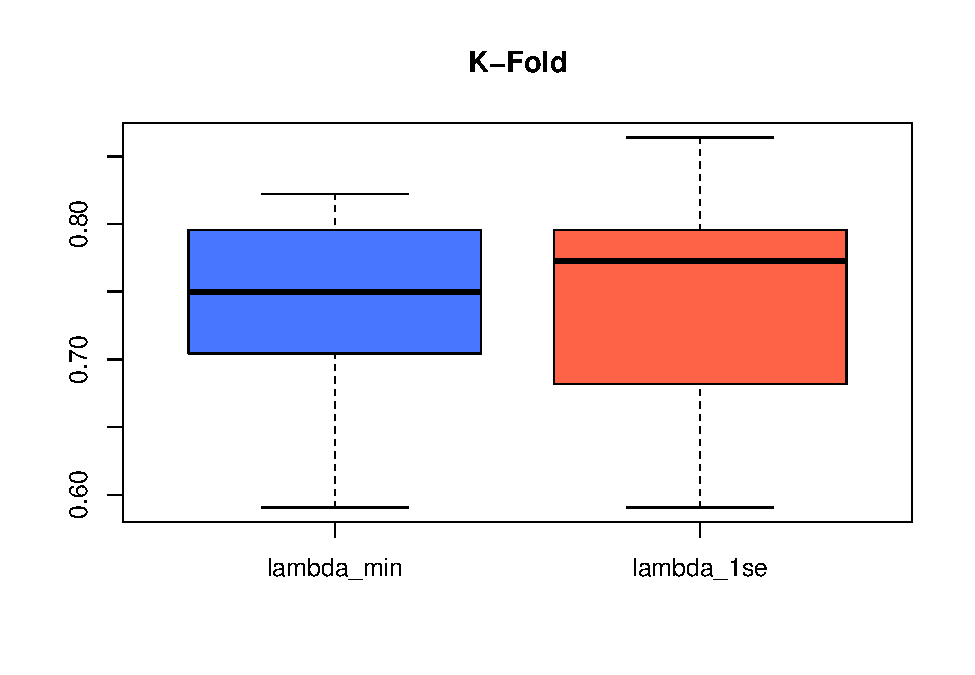
\includegraphics{TP3_MERR_HABBOU_KHIDOUR_files/figure-latex/unnamed-chunk-62-1} \end{center}

In our case we did two 10-Folds with \(\lambda_{min}\) and
\(\lambda_{1se}\). By looking at the boxplots we can see that the median
of our accuracy in between \(75\,\%\) and \(80\,\%\) for the two models.
But we can clearly observe that the box for \(\lambda_{1se}\) is higher
than the one for \(\lambda_{min}\) which means in generally we will have
a better accuracy by using \(\lambda_{1se}\). More than that, we know
that with \(\lambda_{1se}\) we are having a larger penalization than
with \(\lambda_{min}\) which explains why we have a larger interquartile
range and a larger distance between the minimum and the maximum.

\hypertarget{conclusion}{%
\section{Conclusion}\label{conclusion}}

At the end of this practical work, we will keep 5 different models.

\begin{itemize}
\tightlist
\item
  The model corresponding to a constant \(reg_none\)
\item
  The model with all the predictors \(reg_all\)
\item
  The models obtained by using the stepwise methodology \(reg_both\)
\item
  The models obtained by using the ridge methodology \(ridge_min\)
\item
  The models obtained by using the lasso methodology \(lasso_min\)
\end{itemize}

Let's compare their accuracy using a K-Fold procedure for Cross
Validation:

\begin{Shaded}
\begin{Highlighting}[]
\NormalTok{kfold\_none }\OtherTok{\textless{}{-}} \ControlFlowTok{function}\NormalTok{(k) }\CommentTok{\# k is here the number of folds}
\NormalTok{\{}
  \CommentTok{\# create a vector of length number of folds}
\NormalTok{  performance }\OtherTok{\textless{}{-}} \FunctionTok{vector}\NormalTok{(}\AttributeTok{length =}\NormalTok{ k)}
  \CommentTok{\# create a sequence from 1 to k}
\NormalTok{  folds }\OtherTok{\textless{}{-}} \FunctionTok{cut}\NormalTok{(}\FunctionTok{seq}\NormalTok{(}\DecValTok{1}\NormalTok{,}\FunctionTok{nrow}\NormalTok{(diabetes\_data)), }\AttributeTok{breaks =}\NormalTok{ k, }\AttributeTok{labels =} \ConstantTok{FALSE}\NormalTok{)}
  \CommentTok{\# perform k fold cross validation}
  \ControlFlowTok{for}\NormalTok{(i }\ControlFlowTok{in} \DecValTok{1}\SpecialCharTok{:}\NormalTok{k)}
\NormalTok{  \{}
    \CommentTok{\# split data by fold}
\NormalTok{    index }\OtherTok{\textless{}{-}} \FunctionTok{which}\NormalTok{(folds }\SpecialCharTok{==}\NormalTok{ i, }\AttributeTok{arr.ind =} \ConstantTok{TRUE}\NormalTok{)}
\NormalTok{    test\_data }\OtherTok{\textless{}{-}}\NormalTok{ diabetes\_data[index,]}
\NormalTok{    train\_data }\OtherTok{\textless{}{-}}\NormalTok{ diabetes\_data[}\SpecialCharTok{{-}}\NormalTok{index,]}
    \CommentTok{\# train the logistic regression on the train data set}
\NormalTok{    reg\_log }\OtherTok{\textless{}{-}} \FunctionTok{glm}\NormalTok{(YBin }\SpecialCharTok{\textasciitilde{}} \DecValTok{1}\NormalTok{, }\AttributeTok{family =}\NormalTok{ binomial, }\AttributeTok{data =}\NormalTok{ train\_data)}
    \CommentTok{\# make predictions}
\NormalTok{    prediction }\OtherTok{\textless{}{-}} \FunctionTok{predict}\NormalTok{(reg\_log, test\_data)}
    \CommentTok{\# compute confusion matrix}
\NormalTok{    confusion\_matrix }\OtherTok{\textless{}{-}} \FunctionTok{table}\NormalTok{(}\FunctionTok{as.numeric}\NormalTok{(prediction }\SpecialCharTok{\textgreater{}} \FloatTok{0.5}\NormalTok{), diabetes\_data[index,]}\SpecialCharTok{$}\NormalTok{YBin)}
    \CommentTok{\# compute the performance}
\NormalTok{    performance[i] }\OtherTok{\textless{}{-}}\NormalTok{ confusion\_matrix[}\DecValTok{1}\NormalTok{,}\DecValTok{2}\NormalTok{] }\SpecialCharTok{/} \FunctionTok{nrow}\NormalTok{(test\_data)}
\NormalTok{  \}}
  \FunctionTok{return}\NormalTok{ (performance)}
\NormalTok{\}}
\end{Highlighting}
\end{Shaded}

\begin{Shaded}
\begin{Highlighting}[]
\NormalTok{kfold\_step }\OtherTok{\textless{}{-}} \ControlFlowTok{function}\NormalTok{(k) }\CommentTok{\# k is here the number of folds}
\NormalTok{\{}
  \CommentTok{\# create a vector of length number of folds}
\NormalTok{  performance }\OtherTok{\textless{}{-}} \FunctionTok{vector}\NormalTok{(}\AttributeTok{length =}\NormalTok{ k)}
  \CommentTok{\# create a sequence from 1 to k}
\NormalTok{  folds }\OtherTok{\textless{}{-}} \FunctionTok{cut}\NormalTok{(}\FunctionTok{seq}\NormalTok{(}\DecValTok{1}\NormalTok{,}\FunctionTok{nrow}\NormalTok{(diabetes\_data)), }\AttributeTok{breaks =}\NormalTok{ k, }\AttributeTok{labels =} \ConstantTok{FALSE}\NormalTok{)}
  \CommentTok{\# perform k fold cross validation}
  \ControlFlowTok{for}\NormalTok{(i }\ControlFlowTok{in} \DecValTok{1}\SpecialCharTok{:}\NormalTok{k)}
\NormalTok{  \{}
    \CommentTok{\# split data by fold}
\NormalTok{    index }\OtherTok{\textless{}{-}} \FunctionTok{which}\NormalTok{(folds }\SpecialCharTok{==}\NormalTok{ i, }\AttributeTok{arr.ind =} \ConstantTok{TRUE}\NormalTok{)}
\NormalTok{    test\_data }\OtherTok{\textless{}{-}}\NormalTok{ diabetes\_data[index,]}
\NormalTok{    train\_data }\OtherTok{\textless{}{-}}\NormalTok{ diabetes\_data[}\SpecialCharTok{{-}}\NormalTok{index,]}
    \CommentTok{\# train the logistic regression on the train data set}
\NormalTok{    reg\_log }\OtherTok{\textless{}{-}} \FunctionTok{step}\NormalTok{(}\FunctionTok{glm}\NormalTok{(YBin }\SpecialCharTok{\textasciitilde{}}\NormalTok{ ., }\AttributeTok{family =}\NormalTok{ binomial, }\AttributeTok{data =}\NormalTok{ train\_data), }\AttributeTok{direction =} \StringTok{"both"}\NormalTok{, }\AttributeTok{trace =} \ConstantTok{FALSE}\NormalTok{)}
    \CommentTok{\# make predictions}
\NormalTok{    prediction }\OtherTok{\textless{}{-}} \FunctionTok{predict}\NormalTok{(reg\_log, test\_data)}
    \CommentTok{\# compute confusion matrix}
\NormalTok{    confusion\_matrix }\OtherTok{\textless{}{-}} \FunctionTok{table}\NormalTok{(}\FunctionTok{as.numeric}\NormalTok{(prediction }\SpecialCharTok{\textgreater{}} \FloatTok{0.5}\NormalTok{), diabetes\_data[index,]}\SpecialCharTok{$}\NormalTok{YBin)}
    \CommentTok{\# compute the performance}
\NormalTok{    performance[i] }\OtherTok{\textless{}{-}}\NormalTok{ (confusion\_matrix[}\DecValTok{1}\NormalTok{,}\DecValTok{1}\NormalTok{] }\SpecialCharTok{+}\NormalTok{ confusion\_matrix[}\DecValTok{2}\NormalTok{,}\DecValTok{2}\NormalTok{]) }\SpecialCharTok{/} \FunctionTok{nrow}\NormalTok{(test\_data)}
\NormalTok{  \}}
  \FunctionTok{return}\NormalTok{ (performance)}
\NormalTok{\}}
\end{Highlighting}
\end{Shaded}

\begin{Shaded}
\begin{Highlighting}[]
\FunctionTok{boxplot}\NormalTok{(}\FunctionTok{kfold\_none}\NormalTok{(}\DecValTok{10}\NormalTok{), }\FunctionTok{kfold\_all}\NormalTok{(}\DecValTok{10}\NormalTok{), }\FunctionTok{kfold\_step}\NormalTok{(}\DecValTok{10}\NormalTok{), }\FunctionTok{kfold\_ridge}\NormalTok{(}\DecValTok{10}\NormalTok{, cv\_ridge}\SpecialCharTok{$}\NormalTok{lambda.min), }\FunctionTok{kfold\_lasso}\NormalTok{(}\DecValTok{10}\NormalTok{, cv\_lasso}\SpecialCharTok{$}\NormalTok{lambda.min),}
        \AttributeTok{main =} \StringTok{"10{-}Fold for 5 different models"}\NormalTok{, }
        \AttributeTok{names =} \FunctionTok{c}\NormalTok{(}\StringTok{"Null"}\NormalTok{, }\StringTok{"Full"}\NormalTok{, }\StringTok{"Stepwise"}\NormalTok{, }\StringTok{"Ridge Min"}\NormalTok{, }\StringTok{"Lasso Min"}\NormalTok{),}
        \AttributeTok{col =} \FunctionTok{c}\NormalTok{(}\StringTok{"mediumorchid3"}\NormalTok{, }\StringTok{"royalblue3"}\NormalTok{, }\StringTok{"tomato1"}\NormalTok{, }\StringTok{"goldenrod2"}\NormalTok{, }\StringTok{"seagreen"}\NormalTok{))}
\end{Highlighting}
\end{Shaded}

\begin{center}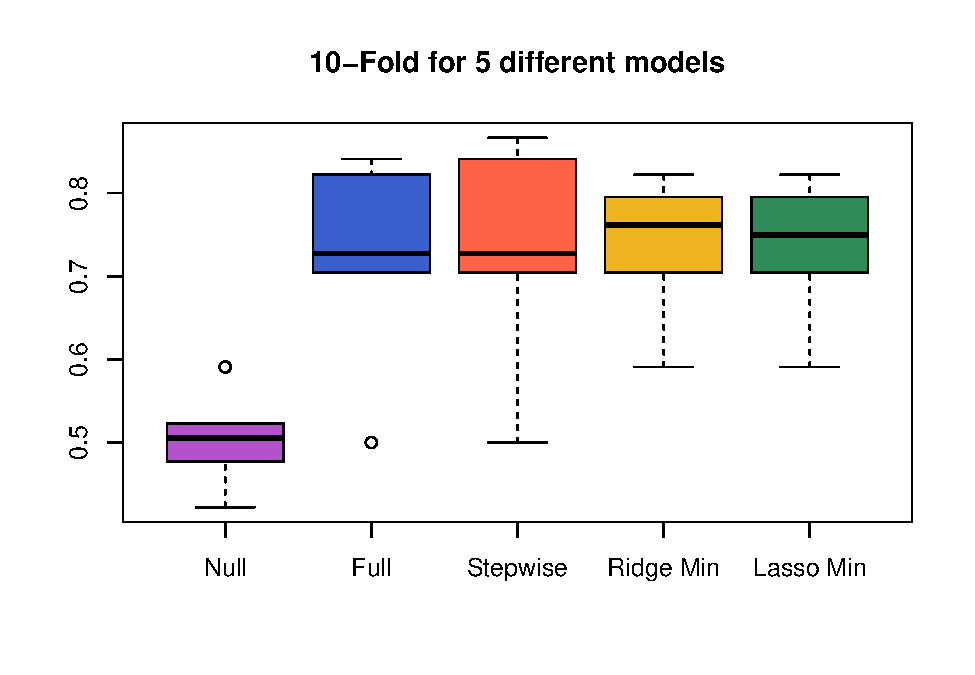
\includegraphics{TP3_MERR_HABBOU_KHIDOUR_files/figure-latex/unnamed-chunk-65-1} \end{center}

By looking at the boxplots we can compare between all the models we did
in this practical work:

\begin{itemize}
\item
  We can notice the presence of outliers;
\item
  The Null model has the lowest accuracy because he doesn't take in
  count any co-variables;
\item
  The Stepwise model has a very small minimum value which is near to the
  median of the Null model;
\item
  The Full and Stepwise models have a better accuracy than the Null
  model but their median are lower than the median for Ridge and Lasso,
  we can explain that by the fact that Ridge and Lasso are applying
  penalization in order to avoid overfitting so it has a better
  predictive power on new data set which is the case when doing K-Fold
  Cross Validation;
\item
  For Ridge and Lasso we can clearly see that they have the best
  accuracy but we can observe than the interquartile range and the
  distance between min and max values are larger for Ridge than for
  Lasso because Lasso does variable selection. Generally, when we have
  many small or medium sized effects we should go with Ridge. If we have
  only a few variables with a medium or large effect, we should go with
  Lasso;
\item
  ``Ridge regression does a proportional shrinkage. Lasso translates
  each coefficient by a constant factor, truncating at zero.'' from
  \textbf{The Elements of Statistical Learning: Data Mining, Inference,
  and Prediction. Hastie, Tibshirani, Friedman}.
\end{itemize}

\end{document}
